\documentclass[12pt]{article}
\usepackage[a4paper]{geometry}
\usepackage[dvipsnames]{xcolor}
\usepackage{lipsum}
\usepackage{framed}
\usepackage{graphicx}
\usepackage{afterpage}
\usepackage[spanish]{babel}
\usepackage[utf8]{inputenc}
\usepackage{titlesec}
\usepackage{colortbl}
\usepackage{xcolor}
\usepackage{cite}

\usepackage{enumerate}
\usepackage{multirow}
\usepackage{graphics}
\usepackage{appendix}
\usepackage[nottoc]{tocbibind}
\addto\captionsspanish{
  \renewcommand{\refname}{Bibliografía}
}

\usepackage{tikz}
\usetikzlibrary{shapes,arrows}
\usepackage{caption}

\captionsetup{
  font=small,              % Tamaño pequeño, fuente LM Roman (por defecto)
  labelfont=bf,            % "Figura X." en negrita
  textfont=it,             % Descripción en cursiva (opcional)
  labelsep=period,         % Punto en lugar de dos puntos
  justification=centering,
  skip=0pt
}

\captionsetup[table]{
  name=Tabla,
  font=small,
  labelfont={bf},
  textfont=it,
  labelsep=period,
  justification=centering,
  position=top            % Captions de tablas arriba
}
\usepackage{subcaption}
\usepackage{amsmath,amsthm,amssymb,mathrsfs} 
\usepackage[final]{pdfpages}
\usepackage[]{placeins,flafter}
\usepackage[none]{hyphenat} \sloppy
\usepackage{xcolor}
\usepackage{adjustbox}
\geometry{top=2.5cm, bottom=2.5cm, left=2.5cm, right=2.5cm}
\usepackage[hidelinks]{hyperref}


% Configuramos el formato de la sección
\titleformat{\section}
  {\normalfont\Large\bfseries} % Estilo del texto
  {\thesection}                % Etiqueta (el número)
  {1em}                        % Espacio entre número y título
  {}                           % Código antes del título
  [{\titlerule[1.2pt]}]        % Código después: la línea (pegada al título)


\titlespacing*{\section}{0pt}{3.5ex plus 1ex minus .2ex}{2pc}


\newcommand{\sectionbreak}{\clearpage} % Requiere el paquete titlesec
\hypersetup{
    colorlinks=true,
    linkcolor=black,      % Color de enlaces internos
    citecolor=blue,       % Color de las citas ← AQUÍ
    filecolor=magenta,
    urlcolor=cyan,
}
\usepackage{chngcntr}
\counterwithin{figure}{section}
\counterwithin{table}{section}
\counterwithin{equation}{section}

\addto\captionsspanish{
  \renewcommand{\listfigurename}{Lista de Figuras}
  \renewcommand{\listtablename}{Lista de Tablas}
  \def\acknowledgmentsname{Agradecimientos}
}
% --- Configuración de Acrónimos ---
\usepackage[acronym, toc, section=section]{glossaries} 
\makeglossaries

% Definición acronimos
\newacronym{imu}{IMU}{Inertial Measurement Unit}
\newacronym{ble}{BLE}{Bluetooth Low Energy}
\newacronym{pcb}{PCB}{Printed Circuit Board}
\newacronym{tfg}{TFG}{Trabajo Fin de Grado}
\newacronym{adc}{ADC}{Analog to Digital Converter}
\newacronym{dac}{DAC}{Digital to Analog Converter}

\begin{document}
\definecolor{light-gray}{gray}{0.87}  

\begin{titlepage}

\vspace*{-4mm}
\begin{figure}[!h]
  \centering
	
\includegraphics[width=69.62mm]{Imagenes/UnizarLogo}
\end{figure}

\vspace*{10mm}

\fontsize{28pt}{28pt}\selectfont
\begin{center}
\setlength{\fboxsep}{3.4mm}
\adjustbox{minipage=14.4cm,cfbox=black,center}{\begin{center} Trabajo Fin de Máster \end{center}}
\end{center}
\vspace*{5mm}

\fontsize{16pt}{16pt}\selectfont
\center{MASTER EN FÍSICA Y TECNOLOGÍAS FÍSICAS}


\vspace*{18.7mm}

\fontsize{20pt}{20pt}\selectfont
\begin{center}
\textbf{Sistema háptico basado en estimulación electrotáctil para captura de movimiento e interacción hombre-máquina }
\end{center}
\baselineskip 20pt

\vspace*{1cm} 
\baselineskip 36pt
\begin{center}
\fontsize{12pt}{12pt}\selectfont
\center{\rm  Autor}

\vspace*{1mm} 
\fontsize{18pt}{18pt}\selectfont
\center{Unax Arregi Ballestero}
\vspace*{1cm}
\baselineskip 36pt
\fontsize{12pt}{12pt}\selectfont
\center{\rm  Directores}
\vspace*{1mm}
\fontsize{14pt}{14pt}\selectfont
\center{Nicolás Medrado Marqués}
\center{Belén Calvo López}
\end{center}

\setcounter{footnote}{1}

\vspace*{26.45mm}
\fontsize{12pt}{12pt}\selectfont
\begin{center}
FACULTAD DE CIENCIAS\\
\vspace{3.5mm}
Departamento de Ingeniería Electronica y Comunicaciones\\
\vspace{3.5mm}
20 de Junio de 2026\\
\end{center}


\renewcommand{\thefootnote}{\arabic{footnote}}
\pagenumbering{gobble}
\end{titlepage}

\pagenumbering{roman}

\phantomsection
\addcontentsline{toc}{section}{\acknowledgmentsname}
\section*{\acknowledgmentsname} 

Especial gracias a MI por creer en MI y constantemente apoyar a MI. Sin MI jamas podria haber hecho todo esto.

\listoffigures        % Índice de figuras
\listoftables         % Índice de tablas


\printglossary[type=\acronymtype, title={Lista de Acrónimos}]
\clearpage

%------------------ ÍNDICE ------------------
\newpage

\tableofcontents
\newpage

\pagenumbering{arabic}

%%%%%%%%%%%%%%%%%%%%%%%%%%%%%%%
%------------------ CONTENIDO ------------------
\section{Introducción}

La progresiva miniaturización de la electrónica y el aumento de la capacidad de procesamiento en sistemas embebidos han impulsado el desarrollo de nuevas formas de interacción entre humanos y dispositivos tecnológicos. En particular, las interfaces hápticas han cobrado especial relevancia en los últimos años, al permitir añadir el sentido del tacto como canal de comunicación con sistemas digitales, complementando los tradicionales estímulos visuales y auditivos. Esta tendencia resulta especialmente interesante en aplicaciones de realidad virtual, teleoperación, asistencia a la discapacidad y control gestual avanzado.

Dentro de este marco, el presente Trabajo Fin de Máster se plantea como una continuación directa del Trabajo Fin de Grado llevado a cabo por Jorge Cuartero \cite{TFG}, en el que se abordó una primera aproximación al uso de sistemas vestibles para la captura del movimiento de la mano y su utilización como interfaz de control remoto mediante un \textit{dataglove}. A partir de esa base inicial, el objetivo actual consiste en avanzar hacia una integración más completa del sistema, incorporando retroalimentación háptica mediante estimulación electrotáctil y mejorando tanto el procesamiento embebido como la conectividad inalámbrica del dispositivo.

El núcleo del desarrollo se centra en un guante háptico capaz de combinar adquisición de movimiento, procesamiento local de datos y generación de sensaciones táctiles en la mano del usuario. Para ello se emplea un microcontrolador con capacidad de comunicación inalámbrica, una unidad de medida inercial (\gls{imu}) para la estimación de la orientación espacial y un sistema de estimulación eléctrica diseñado para generar sensaciones referidas en la zona palmar sin obstaculizar la manipulación natural de objetos. Así, se consigue mantener funcionalidad manual a la misma vez que se introduce un canal adicional de información sensorial.

El sistema resultante pretende servir como plataforma experimental para el estudio de interfaces hápticas portables y su aplicación a tareas de control e interacción virtual. La combinación de procesamiento embebido, adquisición sensorial y estimulación táctil en un único dispositivo portátil abre la puerta a interfaces más naturales, compactas y eficientes, donde parte del procesamiento se realiza localmente, reduciendo latencias y mejorando la autonomía del sistema.

A lo largo de la memoria, primeramente, se presenta el fundamento del sistema de estimulación electrotáctil y los criterios de diseño adoptados para lograr sensaciones localizadas en la mano. Después se describe el hardware del dispositivo, incluyendo el microcontrolador, la instrumentación sensorial y la electrónica necesaria. A continuación, se detalla el procesamiento de los datos de orientación y la integración de la información adquirida, junto con la caracterización experimental del sistema háptico. Finalmente, como aplicación del trabajo, se implementa el guante como un sustituto del mando de control de un dron, usando la comunicación inalámbrica brindada por el microcontrolador y empleando la parte háptica como un canal de información para conocer la telemetría del dron sin usar pantallas. Para concluir, se entabla una discusión de las limitaciones actuales y posibles líneas futuras de desarrollo.


\section{Generación de sensación táctil en la zona palmar de la mano}

Para poder crear sensación táctil en la mano, el objetivo es estimular los nervios que la atraviesan con una corriente determinada. Tanaka et al. \cite{Tanaka2023} diseñaron este sistema tratando de generar estas sensaciones en la zona palmar de la mano sin obstruir la misma, preservando así la destreza manual y la capacidad de interactuar con objetos físicos. Para lograrlo, se emplea una técnica basada en \textit{sensaciones referidas}, donde la estimulación eléctrica aplicada en una zona (el dorso de la mano) provoca percepciones somatosensoriales en una zona distal (la palma).

A continuación, se describen los cinco desafíos técnicos identificados en la literatura analizada y las soluciones de diseño implementadas para alcanzar una estimulación precisa en 11 puntos de la zona palmar.

\paragraph{Desafío 1: Selección del punto de estimulación anatómica:} 

Aunque los nervios mediano y cubital recorren el antebrazo y la muñeca, la estimulación en estos puntos se ve limitado debido a que los nervios se encuentran agrupados o empaquetados. Esto impide la activación selectiva de dedos individuales sin generar interferencias entre ellos. 

Se optó por situar los electrodos en el dorso de la mano, ya que tras cruzar la muñeca, los nervios digitales se ramifican hacia cada dedo de forma independiente, haciendo posible un control individualizado. Esta diferencia anatómica en la distribución de los nervios se ilustra en la Figura~\ref{fig:nervios_dorso}.


\paragraph{Desafío 2: Profundidad de penetración de la corriente}
Una disposición convencional de electrodos (ánodo y cátodo próximos sobre el dorso) resulta ineficaz, ya que la corriente fluye de forma superficial, estimulando solo los nervios dorsales. El principio físico aplicado aquí es que la profundidad de penetración de la corriente es proporcional a la distancia entre los electrodos. Para alcanzar los nervios palmares desde el dorso, se diseñó un sistema con una gran distancia inter-electrodo, permitiendo que la corriente atraviese de manera transversal el tejido de la mano. Esta elección de diseño se ilustra en la Figura~\ref{fig:nervios_dorso}.

\begin{figure}[htbp]
    \centering
    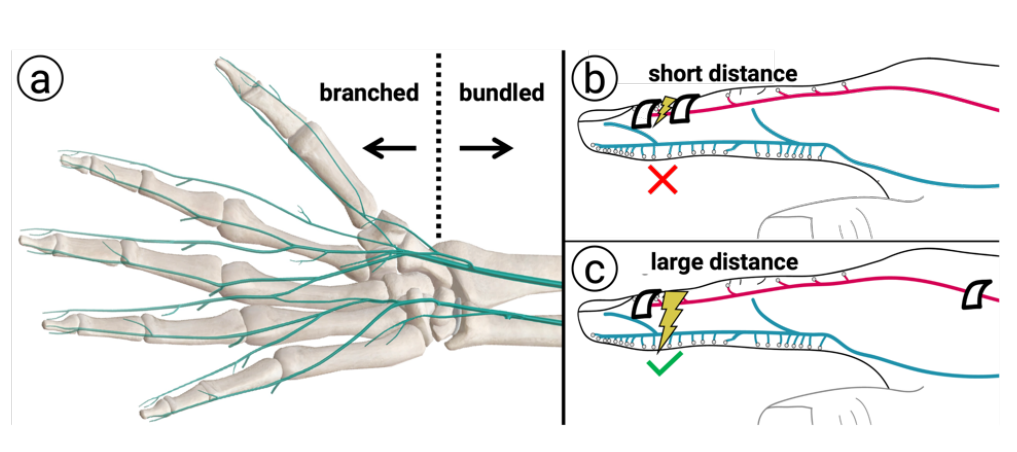
\includegraphics[width=0.8\textwidth]{Imagenes/nervios.png}
    \caption[Diferencia de agrupación nerviosa]{Diferencia entre la agrupación nerviosa en la muñeca y la ramificación en el dorso de la mano para la estimulación individual de dedos. Adaptado de \cite{Tanaka2023}.}
    \label{fig:nervios_dorso}
\end{figure}

\paragraph{Desafío 3: Asimetría sensorial y umbrales de estimulación}
La estimulación desde el dorso activa teóricamente tanto la zona dorsal como la palmar, lo que podría generar sensaciones confusas. Para resolver este conflicto, se aprovecha la diferencia entre número de neuronas que tienen las distintas partes de la mano: la zona palmar posee aproximadamente 18,000 mecanorreceptores, frente a solo 300 en la zona dorsal. 

Aprovechando esta diferencia, al calibrar la intensidad de la corriente, es posible superar el umbral de percepción palmar manteniéndose por debajo del umbral dorsal, haciendo que la sensación en la palma sea la única percibida por el usuario (ver Figura~\ref{fig:umbrales_sensibilidad}).

\paragraph{Desafío 4: Focalización de la sensación y polaridad}
Se observó que los electrodos situados en el dorso de los dedos generan sensaciones desplazadas (\textit{offset}) respecto a la ubicación deseada en la palma; específicamente, no lograban estimular las falanges distales. 

La solución implementada consistió en la manipulación de la polaridad. Mientras que la estimulación anódica es el estándar, se implementó una inversión a estimulación catódica para los electrodos de las falanges distales. Esto permite adelantar la ubicación de la sensación hacia la punta de los dedos, permitiendo la estimulación precisa del pulpejo desde el dorso.

\begin{figure}[htbp]
    \centering
    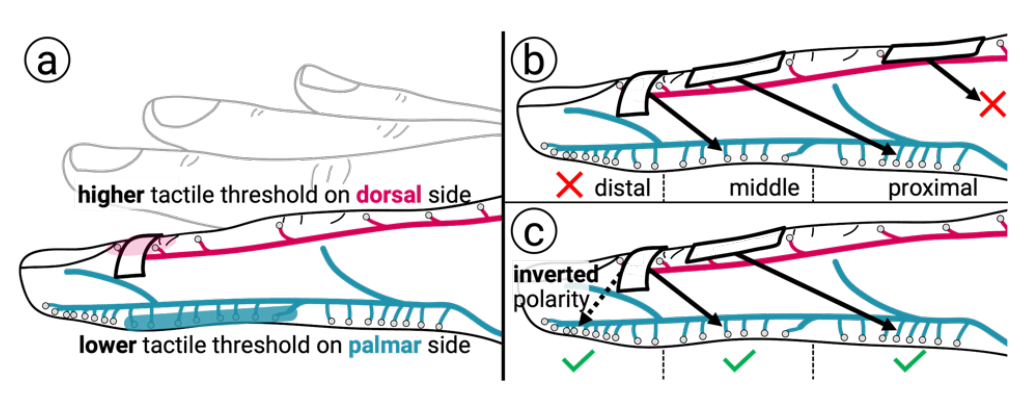
\includegraphics[width=0.8\textwidth]{Imagenes/umbrales.png}
    \caption[Asimetría de umbrales en la mano]{(a) El umbral táctil para la estimulación eléctrica es significativamente más bajo en el lado palmar que en el lado dorsal. (b, c) El uso de ambas polaridades (anódica y catódica) para el electrodo fijado a la punta del dedo permite la estimulación del pulpejo.}
    \label{fig:umbrales_sensibilidad}
\end{figure}

\paragraph{Desafío 5: Mitigación de interferencias inter-digitales}
Debido a que el nervio mediano inerva los dedos pulgar, índice y medio, mientras que el nervio cubital (ulnar) inerva el anular y meñique, el uso de un único electrodo de tierra general provocaba sensaciones referidas no deseadas en dedos adyacentes. 

El diseño final solventa este problema mediante el uso de dos electrodos de tierra independientes, uno para cada nervio. Al conmutar el flujo de corriente hacia la tierra correspondiente según el dedo objetivo, se logra una selectividad total, resultando en un sistema capaz de generar sensaciones en 11 puntos diferenciados de la mano sin obstrucción palmar alguna, tal como se detalla en el esquema de la Figura~\ref{fig:disposicion_electrodos}.

\begin{figure}[htbp]
    \centering
    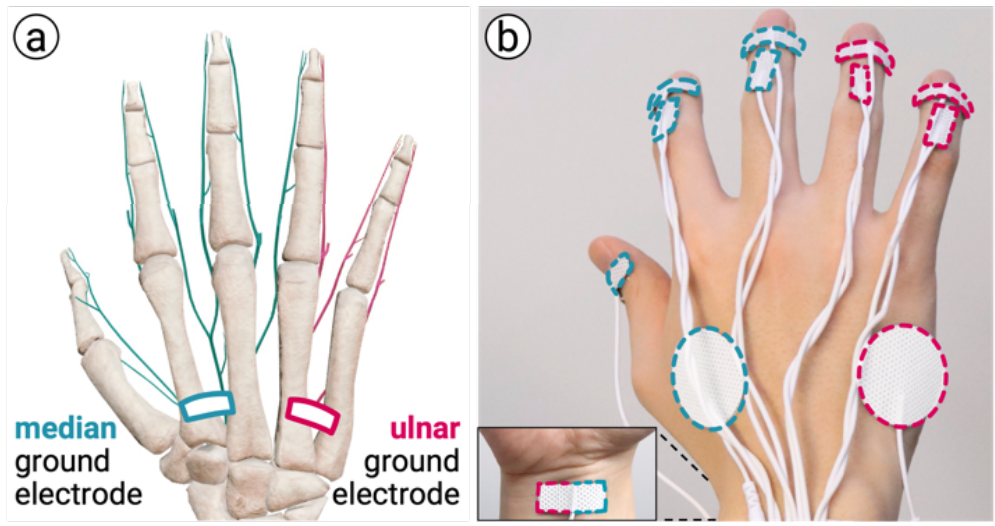
\includegraphics[width=0.8\textwidth]{Imagenes/disposicionfinal.png}
    \caption[Configuración final del sistema háptico]{Configuración final de electrodos con doble toma de tierra para evitar interferencias entre los nervios mediano y cubital.}
    \label{fig:disposicion_electrodos}
\end{figure}


\section{Interfaz hardware}

El sistema completo para poder llevar a cabo el objetivo propuesto se monta en un guante, que se muestra en la Figura \ref{fig:montaje_completo}. Se distinguen los siguientes componentes: en cada dedo, del anular al meñique, sujetas por unas pequeñas piezas, fijamos bandas piezorresistivas que nos permitirán determinar su flexión. En la parte inferior se encuentra la PCB, capaz generar corrientes controladas por voltaje y programadas mediante un potenciometro digital. En la parte inferior de la placa, se encuentran los conectores hembra donde se introducen los electrodos conectados a la mano. La información proporcionada por las bandas se introduce en un Raspberry RP2040 Connect, alojado en una caja central fijada a la muñeca. A la misma vez, este dispositivo se encarga de la generación de señales eléctricas que pasan por la PCB.

\begin{figure}[htbp]
    \centering
    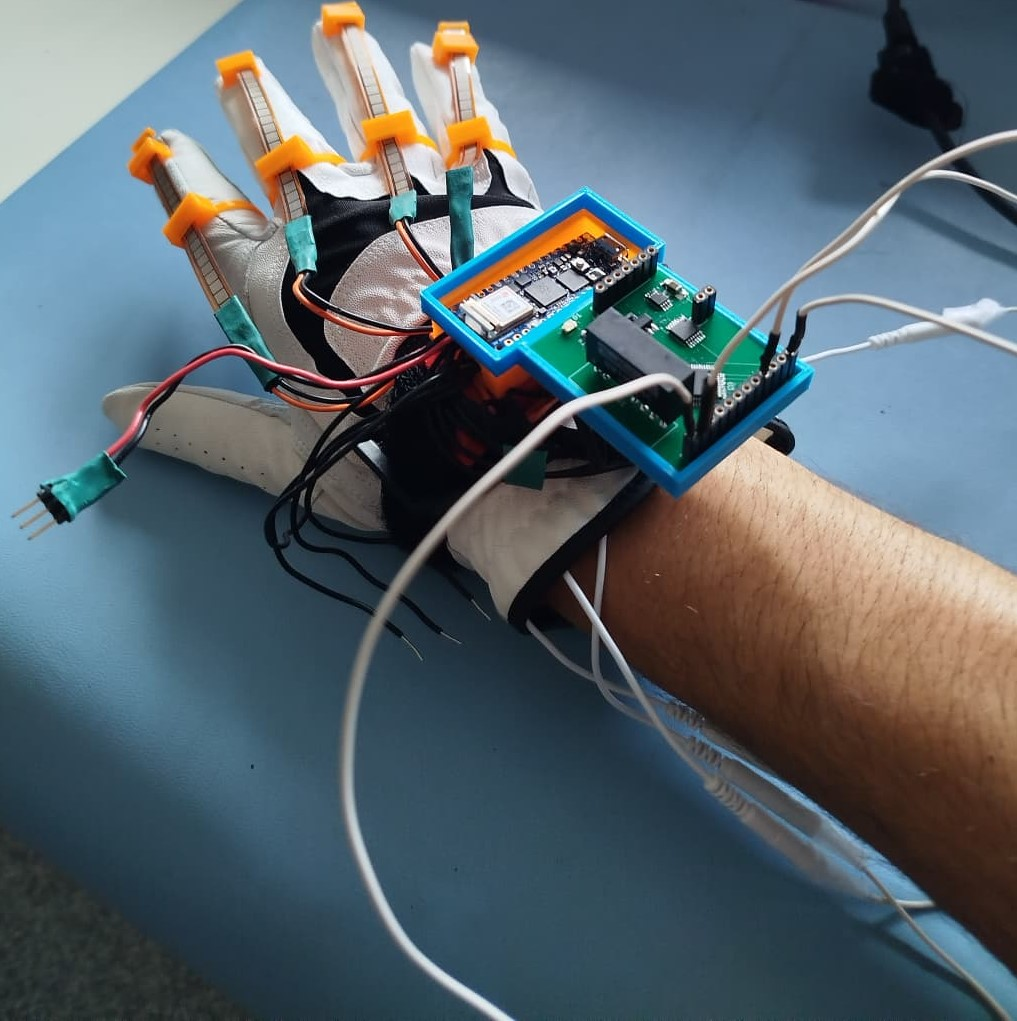
\includegraphics[width=0.5\textwidth]{Imagenes/montaje_completo.jpeg}
    \caption[Montaje final del sistema háptico]{Montaje final del sistema háptico y de captura de movimiento}
    \label{fig:montaje_completo}
\end{figure}


\subsection{Arduino Nano RP2040 Connect}
El microcontrolador usado para el trabajo será un módulo Arduino RP2040 Connect \cite{Arduino2040}, que incorpora un microcontrolador Raspberry Pi Pic. Este controlador proporciona una gran potencia de cálculo, un factor que será relevante en el procesamiento de datos que se llevará a cabo para la estimación de la orientación. Además tiene un modulo wifi, que se usará para la comunicación en la interfaz de control en la sección \ref{sec:dron}.

En cuanto a las especificaciones generales, el RP2040 Connect opera a 3.3 V. Consta de un microcontrolador Raspberry Pi Pico (133 MHz de reloj, 256 kB de memoria SRAM) con 8 entradas analógicas (configuradas como convertidores analógico-digitales o  \gls{adc}, de las que 4 estarían destinadas a la adquisición de las posiciones de los dedos. Cuenta además con una \gls{imu} de 6 ejes, modelo LSM6DSOXTR \cite{LSM6DSOX}.
\

\subsubsection{Módulo LSM6DSOXTR}

Este módulo \cite{LSM6DSOX} consta de un acelerómetro y un giróscopo, proporcionando así información de 6 ejes (3 de aceleración y 3 de rotación espacial). Aunque ambos pueden operar a distintos fondos de escala y resoluciones, la librería utilizada (Arduino\_LSM6DSOX \cite{LibreriaLSM6DSOX}) viene configurada con una sensibilidad de 0.122 mg/LSB (siendo g la aceleración de la gravedad y LSB el bit menos significativo o Least Significant Bit) para el acelerómetro y una sensibilidad de 0.07 dps/LSB para el giróscopo (donde dps son Degrees per second, grados por segundo), valores adecuados para nuestra aplicación
(menores que el propio ruido). Esta librería dispone de dos funciones, una encargada de devolver 3 valores en representación de punto flotante para los tres ejes de la aceleración, y la otra de devolver los 3 valores referentes a la velocidad de rotación en cada eje en el mismo formato.

La frecuencia de medida está fijada en 104 Hz de manera predeterminada por la librería LSM6DSOX. Aunque una alta frecuencia de muestreo era importante para la estimación de la orientación mediante integración del giroscopio \cite{TFG}, para el método que se utilizará en este trabajo con esta tasa de muestreo se obtendrá un resultado que no se verá limitado por este valor. De todos modos, con esta configuración un ciclo de medida y procesado de nuestro Arduino no podrá durar más de 10  para que no se solapen medidas de la \gls{imu}, forzando a optimizar los tiempos de cada parte del procesado.

\subsubsection{Módulo de conectividad inalámbrica NINA-W102}

La comunicación inalámbrica del guante se implementa a través del módulo u-blox NINA-W102 \cite{NINA-W102}, integrado directamente en la placa Arduino Nano RP2040 Connect. Su arquitectura interna aloja un microprocesador de doble núcleo ESP32 dedicado en exclusiva a la gestión de la pila de protocolos de red, lo que descarga completamente al procesador principal RP2040 de esta tarea y preserva su capacidad de cómputo para el procesamiento de la \gls{imu}, la lógica de control y el sistema háptico.

El módulo soporta tanto \gls{ble} como Wi-Fi (802.11 b/g/n a 2.4~GHz). Para este diseño se ha optado por Wi-Fi, ya que el volumen de datos a transmitir (orientación de la \gls{imu} más flexión de los cuatro dedos en tiempo real) exige un ancho de banda que \gls{ble} no puede garantizar sin introducir retardos
en el lazo de control con el entorno virtual, a parte de qué usar Wi-Fi será imprescindible debido a las caracteristicas del dron que se operará en la sección \ref{sec:dron}.

\subsection{Sistema de adquisición de posiciones de la mano}
El sistema de determinación de la flexión de los dedos se basa en las bandas piezorresistivas antes mencionadas. Una piezorresistencia es un material o componente que, bajo un esfuerzo mecánico, sufre un cambio en su resistividad. En nuestro caso se usarán los Flex Sensor de Spectra Symbol \cite{Flex-Sensor}, caracterizados por valores nominales entre 7 kΩ y 13 kΩ en reposo, de forma que al ser dobladas, como mínimo duplican su valor resistivo. Como el Arduino no puede medir directamente resistencias, en \cite{TFG} se implementó un circuito auxiliar que permite traducir estos cambios en tensión.

Este circuito consiste en un divisor resistivo formado por una resistencia fija ($R_{\text{fija}}$) en serie con el elemento piezorresistivo ($R_{\text{piezo}}$), alimentado a los 3.3~V proporcionados por el propio microcontrolador. De este modo, las variaciones de resistencia de los sensores se transforman en variaciones de voltaje según la relación:

\begin{equation}
V_{\text{divisor}}(R_{\text{piezo}}) = 3.3 \cdot \frac{R_{\text{fija}}}{R_{\text{piezo}} + R_{\text{fija}}}
\end{equation}

Para maximizar el rango de oscilación de la tensión de salida y optimizar la precisión de la lectura, el valor de $R_{\text{fija}}$ se calcula para cada sensor mediante la media geométrica de sus extremos resistivos:

\begin{equation}
R_{\text{fija}} = \sqrt{R_{\text{max}} \cdot R_{\text{min}}}
\end{equation}

donde $R_{\text{max}}$ y $R_{\text{min}}$ representan las resistencias máxima y mínima medidas en flexión (pico) y extensión (relajado), respectivamente. En el montaje real, se seleccionan los valores comerciales de resistencia fija más cercanos a los óptimos teóricos calculados para el rango de cada dedo. El cálculo con los valores que finalmente se usan en el \textit{dataglove} se detallan en el anexo de \cite{TFG}.

La tensión de salida del divisor se introduce en los pines analógicos del microcontrolador, configurados como entradas del \gls{adc}. Este convertidor opera con una resolución de 10 bits (lo que genera un rango digital de 0 a 1023 cuentas) y un rango de tensión de 0 a 3.3~V, lo que resulta en una resolución de medida de 3.2~mV. Además, el tiempo de adquisición es inferior a 30~$\mu$s, lo que cumple holgadamente con los requisitos de velocidad y tasa de muestreo exigidos para completar un ciclo de nuestro proceso.

\subsection{Circuito de estimulación electrotáctil}

Para poder conseguir estimular los nervios de la mano y generar sensación táctil, según la bibliografía existente en el ámbito \cite{Tanaka2023}, la corriente generada debe ser del orden de pocos miliamperios y, al mismo tiempo, de suficiente tensión como para superar la impedancia de la piel, que según medidas rápidas tomadas en el laboratorio esta en torno al megaohmio. 

Además, según el sistema de electrodos descrito en la sección 2, debe poder conmutar entre 10 canales de estimulación y cambiar entre corriente catódica y anódica según lo requiera la configuración correspondiente, por lo que teniendo todo esto en cuenta el circuito finalmente construido será el de la Figura \ref{fig:circuito_estimulacion}:

\begin{figure}[htbp]
    \centering
    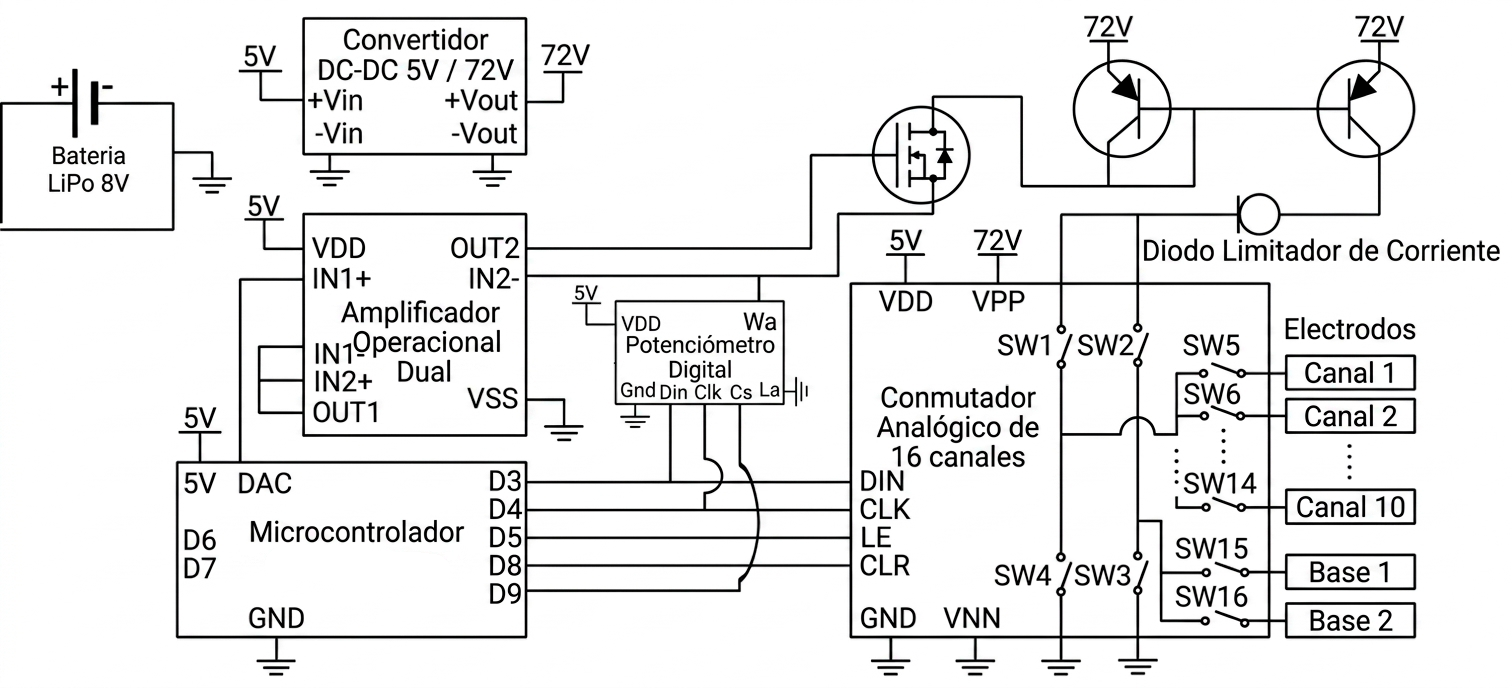
\includegraphics[width=\textwidth]{Imagenes/Circuito_estimulacion.png} % Ajusta el nombre y escala
    \caption{Esquema del circuito de estimulación electrotáctil diseñado para el guante.}
    \label{fig:circuito_estimulacion}
\end{figure}

A diferencia de los diseños previos de la literatura que dependían de reguladores elevadores intermedios y baterías de baja tensión \cite{Tanaka2023}, este circuito se alimenta directamente a través de la batería de 7.4~V con una capacidad de almacenamiento de energía de 1000 mAh conectada al pin $V_{\text{in}}$ del Arduino Nano RP2040 Connect, colocando en el cable que sale a alimentar el sistema un regulador a 5 V constantes. Para la etapa de estimulación, la generación de la alta tensión de 72~V se confía a un convertidor DC-DC modelo NMT0572SC, el cual se alimenta con esta salida regulada de 5~V.

Como este microcontrolador no tiene una salida \gls{dac}, para controlar de manera precisa la intensidad de los impulsos electrotáctiles y adaptarla a los umbrales sensitivos del usuario, se ha sustituido el potenciómetro analógico manual por un potenciómetro digital MAX5413. El microcontrolador gobierna este dispositivo mediante un protocolo basado en SPI, optimizando el uso de pines al compartir las líneas de datos DIN y de reloj CLK con el circuito integrado de conmutación de alta tensión HV2701, requiriendo únicamente una línea adicional para la selección de chip el potenciometro (CS*). La señal digital del microcontrolador se hace pasar por este potenciómetro y se introduce en un amplificador operacional LMV341 conectado a un FET BSS87, configurando una fuente de corriente controlada por voltaje para independizar la señal de la carga. Acto seguido, un espejo de corriente basado en transistores bipolares BJT FCX705 replica esta corriente de referencia y la transfiere hacia la línea de alta tensión (72~V), asegurando un flujo eléctrico constante.

La señal de corriente regulada por esta etapa se inyecta en el conmutador analógico de alta tensión HV2701. Este circuito integrado multiplexa la señal hacia los 10 canales disponibles en la mano y las dos tomas de tierra independientes (Base 1 y Base 2), encargadas de aislar los nervios mediano y cubital. Internamente, una matriz de interruptores actúa a modo de puente en H para invertir dinámicamente la polaridad de la estimulación (catódica o anódica) según los requerimientos específicos de la zona palmar seleccionada.

Debido a la arquitectura del sistema, se aplica una técnica de multiplexación temporal para mitigar las interferencias; de este modo, el integrado HV2701 solo habilita un camino de corriente hacia un único objetivo simultáneamente. Dado que este integrado es capaz de conmutar entre canales en un tiempo de apenas 10~$\mu$s, el firmware del Arduino completa un ciclo secuencial para todos los canales en un intervalo inferior a 10~ms. Puesto que el umbral de discriminación temporal del sentido del tacto humano se sitúa en torno a los 50~ms, el usuario percibe la activación de múltiples puntos de la mano de forma totalmente concurrente a frecuencias de hasta 100~Hz \cite{Tanaka2023}.

Para dotar de seguridad al sistema y evitar accidentes se integra en serie un diodo limitador de corriente (E-452) que actúa como limitador físico si la corriente de salida llega a alcanzar los 4.5~mA, garantizando la inocuidad del guante ante cualquier fallo de ejecución en el microcontrolador. Por último, todo este diseño electrónico se ha plasmado en una PCB que fue diseñada mediante el software KiCad y posteriormente enviada a fabricar para su ensamblaje final, diseño y resultado que se pueden ver en la Figura \ref{fig:diseno_pcb}.


\begin{figure}[htbp]
    \centering
    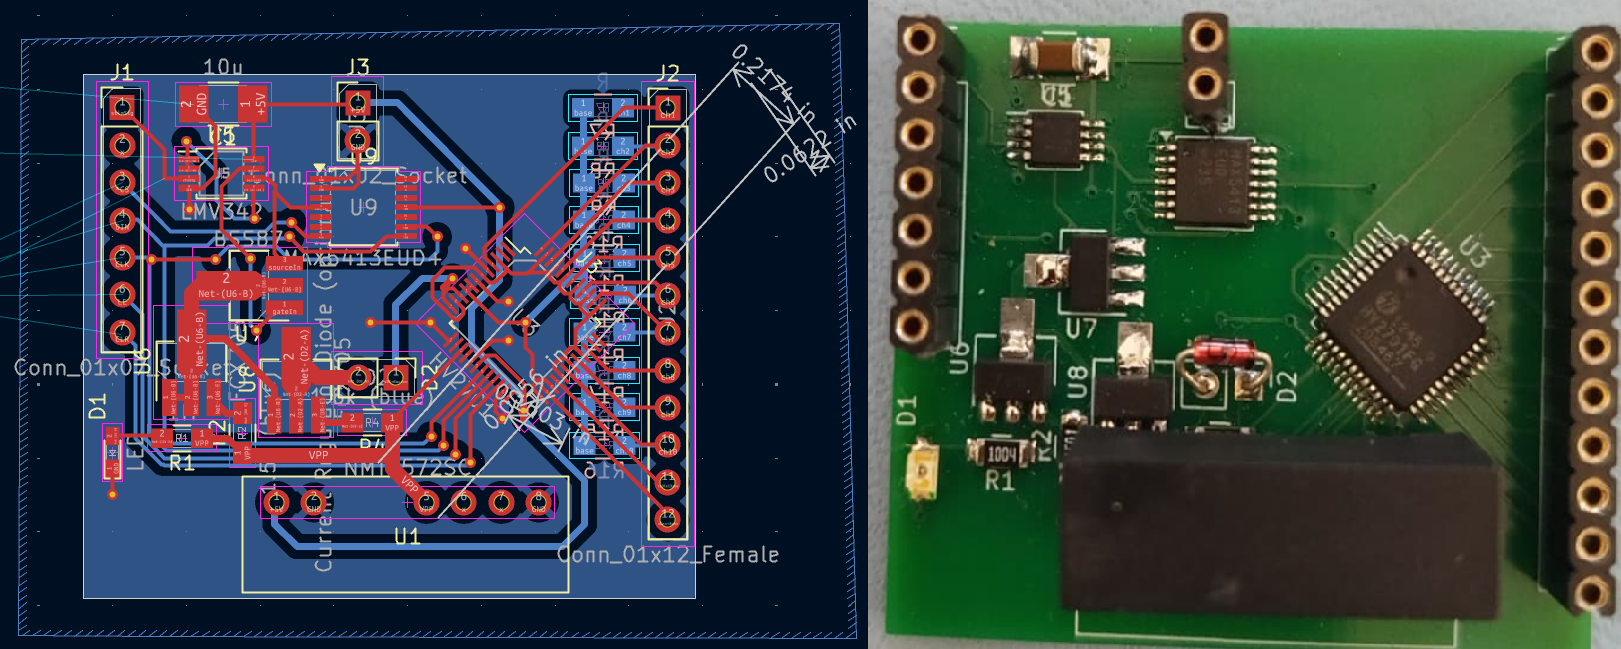
\includegraphics[width=\textwidth]{Imagenes/diseño_pcb.png} % Ajusta el nombre de la imagen y escala
    \caption{Diseño final de la PCB del circuito de estimulación electrotáctil desarrollado en KiCad y resultado final una vez se recibió de la fábrica. Agradecimientos a Diego Antolín por su ayuda con el diseño y a Óscar Lasarte por montar la placa.}
    \label{fig:diseno_pcb}
\end{figure}

\section{Procesamiento de datos: orientación espacial}
El núcleo del procesamiento de datos de la \gls{imu} LSM6DSOXTR reside en la estimación precisa de la orientación del sensor. Anteriormente, se planteaba el sistema de ecuaciones para obtener la expresión de los ángulos de Euler de la orientación, pero haciendo esto, una de las ecuaciones debe de integrar en el tiempo dos de los ejes del giroscopio. Con este método el procesamiento inducia en deriva de uno de los ángulos de manera inevitable \cite{TFG}.

Para este trabajo, se ha implementado un filtro complementario no lineal propuesto por Mahony et al. \cite{Mahony2008}, el cual formula el problema de estimación como una cinemática de observador determinista directamente sobre el grupo ortogonal especial $SO(3)$. Este método utiliza la geometría del grupo de Lie para desacoplar las mediciones del giroscopio del error de actitud reconstruido, buscando una implementación lo más eficiente posible para el hardware disponible.

\subsection{Representación de la orientación: cuaterniones}

Antes de formular el filtro, es necesario elegir cómo representar matemáticamente la orientación del sensor en el espacio tridimensional. La opción más intuitiva son los ya mencionados ángulos de Euler: guiñada $\psi$ (\textit{yaw}), cabeceo $\theta$ (\textit{pitch}) y alabeo $\phi$ (\textit{roll}). Estos presentan una singularidad
conocida como \textit{gimbal lock} cuando dos ejes de rotación se alinean, además de requerir funciones trigonométricas computacionalmente costosas para el RP2040.
Por ello, el filtro opera internamente con cuaterniones unitarios, una representación algebraica que evita estas singularidades y permite actualizar la orientación mediante operaciones aritméticas simples.

Un cuaternión unitario $\mathbf{q}$ queda definido como:

\begin{equation}
\mathbf{q} =
\begin{pmatrix}
q_0 \\ q_1 \\ q_2 \\ q_3
\end{pmatrix},
\qquad \|\mathbf{q}\|=1,
\end{equation}

donde $q_0$ es la parte escalar, asociada al ángulo de rotación, y
$(q_1, q_2, q_3)$ es la parte vectorial, asociada al eje de rotación. La condición de unitariedad garantiza que el cuaternión represente siempre una rotación pura, sin escalado. Cuando se requiere expresar la orientación final en ángulos de Euler para enviarlos al entorno de control, la conversión se realiza a posteriori, de forma que todo el procesamiento interno permanece libre de singularidades.

\subsection{Fusión de acelerómetro y giroscopio}

El giroscopio proporciona la velocidad angular $\boldsymbol{\omega}$, que integrada en el tiempo permite seguir la evolución de la orientación con gran precisión a corto plazo.
Sin embargo, cualquier sesgo (\textit{bias}) estático o deriva lenta en sus lecturas se acumula en la integral, generando un error de orientación que crece sin límite con el tiempo. El acelerómetro, por su parte, mide la aceleración total del sensor; cuando el guante no está sometido a aceleraciones externas apreciables, esta medida queda
dominada por la gravedad terrestre, cuya dirección es conocida en el marco inercial.
Esto permite obtener una referencia absoluta de inclinación, libre de deriva, aunque ruidosa en presencia de movimientos bruscos.

El filtro de Mahony se basa en la complementariedad de ambos sensores: el giroscopio proporciona una estimación dinámica y precisa a corto plazo, mientras que el acelerómetro corrige continuamente la deriva a largo plazo. Para cuantificar cuánto difiere la orientación estimada de la real se define un error vectorial $\mathbf{e}$ mediante el producto vectorial entre la dirección de la gravedad medida por el acelerómetro normalizada y la dirección de la gravedad que el cuaternión actual predice en el marco del sensor \cite{Mahony2008}:

\begin{equation}
\mathbf{e} = \hat{\mathbf{a}} \times \mathbf{v},
\end{equation}

donde $\hat{\mathbf{a}} = \mathbf{a}/\|\mathbf{a}\|$ es la aceleración normalizada y $\mathbf{v}$ es la estimación de la dirección de la gravedad obtenida rotando el vector $[0,0,1]^T$ con el cuaternión actual:

\begin{equation}
\mathbf{v} =
\begin{pmatrix}
2(q_1 q_3 - q_0 q_2) \\
2(q_0 q_1 + q_2 q_3) \\
q_0^2 - q_1^2 - q_2^2 + q_3^2
\end{pmatrix}.
\end{equation}

El producto vectorial produce un vector cuya dirección es el eje en torno al cual debe corregirse la estimación y cuya magnitud es proporcional al ángulo de error. Cuando ambos vectores coinciden, el error es nulo y el filtro no introduce ninguna corrección. Por lo tanto, esta formulación evita la reconstrucción algebraica completa de la actitud, ya que el error se calcula directamente en el espacio del sensor sin pasar por ángulos de Euler.

\subsection{Controlador PI y corrección del bias}

El error $\mathbf{e}$ se utiliza para corregir la velocidad angular antes de integrarla, mediante un controlador proporcional-integral (PI) clásico. La acción proporcional, escalada por la ganancia $K_p$, reacciona inmediatamente al error presente; la acción integral, escalada por $K_i$, acumula el error a lo largo del tiempo y compensa el sesgo estático del giroscopio:

\begin{equation}
\mathbf{e}_{\text{int}}(t) = \mathbf{e}_{\text{int}}(t - \Delta t) + K_i \, \mathbf{e} \, \Delta t,
\end{equation}

\begin{equation}
\boldsymbol{\omega}_c = \boldsymbol{\omega} + K_p \mathbf{e} + \mathbf{e}_{\text{int}}.
\end{equation}

La velocidad angular corregida $\boldsymbol{\omega}_c$ se usa para propagar el cuaternión en el tiempo. La cinemática diferencial del cuaternión unitario establece que:

\begin{equation}
\dot{\mathbf{q}} = \frac{1}{2} \, \mathbf{q} \otimes
\begin{pmatrix} 0 \\ \boldsymbol{\omega}_c \end{pmatrix},
\end{equation}

donde $\otimes$ denota el producto de cuaterniones. Discretizando mediante integración de Euler con paso $\Delta t$:

\begin{equation}
\mathbf{q}_{k+1} = \mathbf{q}_k + \frac{1}{2} \, \mathbf{q}_k \otimes
(0, \boldsymbol{\omega}_c) \, \Delta t,
\end{equation}

lo que, expandido en sus cuatro componentes, resulta en:

\begin{equation}
\begin{aligned}
q_0 &\leftarrow q_0 - \tfrac{\Delta t}{2}(q_1 g_x + q_2 g_y + q_3 g_z), \\
q_1 &\leftarrow q_1 + \tfrac{\Delta t}{2}(q_0 g_x + q_2 g_z - q_3 g_y), \\
q_2 &\leftarrow q_2 + \tfrac{\Delta t}{2}(q_0 g_y - q_1 g_z + q_3 g_x), \\
q_3 &\leftarrow q_3 + \tfrac{\Delta t}{2}(q_0 g_z + q_1 g_y - q_2 g_x),
\end{aligned}
\end{equation}

donde $(g_x, g_y, g_z)$ son las componentes de $\boldsymbol{\omega}_c$. Estas operaciones son básicamente sumas y multiplicaciones de enteros en punto flotante, sin funciones trigonométricas, lo que hace al algoritmo sea adecuado para el RP2040. Tras cada iteración, el cuaternión se renormaliza para mantener la condición de unitariedad y evitar la acumulación de errores numéricos:

\begin{equation}
\mathbf{q} \leftarrow \frac{\mathbf{q}}{\|\mathbf{q}\|}.
\end{equation}

La estabilidad de este esquema de corrección fue demostrada por Mahony et al. \cite{Mahony2008} mediante un análisis de Lyapunov. Utilizando como función candidata la traza de la matriz de error de orientación y el módulo del bias estimado, se prueba que su derivada temporal es semidefinida negativa, lo que garantiza la convergencia
casi global del error de orientación a cero y del bias estimado hacia su valor real.

\subsection{Calibración inicial y recentrado dinámico}

Al encender el guante, antes de comenzar la estimación en régimen permanente, se realiza una fase de calibración en la que el sistema se mantiene en reposo durante la adquisición de $N = 100$ muestras de velocidad angular. El bias inicial del giroscopio se estima como la media de dichas muestras:

\begin{equation}
\mathbf{b}_\omega = \frac{1}{N} \sum_{i=1}^{N} \boldsymbol{\omega}_i,
\end{equation}

y a partir de ese instante, toda medida angular se corrige sustrayendo este valor antes de introducirlo en el filtro. Esta calibración reduce el error inicial del controlador
integral, acelerando la convergencia del filtro.

Además del sesgo del giroscopio, existe un segundo problema práctico: la orientación física del guante en el momento de encendido puede ser arbitraria, lo que haría que el entorno virtual comenzara siempre en una postura diferente. Para resolverlo, una vez completada la   calibración se captura el cuaternión resultante como referencia de
postura neutra, calculando su conjugado:

\begin{equation}
\mathbf{q}_{\text{off}} = (q_0, -q_1, -q_2, -q_3).
\end{equation}

A partir de ese momento, la orientación transmitida al entorno de control no es $\mathbf{q}$ sino la orientación relativa al instante de referencia, obtenida mediante el producto:

\begin{equation}
\mathbf{q}_{\text{rel}} = \mathbf{q}_{\text{off}} \otimes \mathbf{q}.
\end{equation}

Este recentrado garantiza que el sistema arranque siempre en una postura neutra definida por el usuario, independientemente de la orientación física inicial del guante, simplificando enormemente la puesta en marcha y haciendo el dispositivo robusto frente a variaciones en la colocación del guante entre sesiones.


\section{Procesamiento de datos: flexión de los dedos}

A diferencia del bloque anterior, orientado al tratamiento de los datos de la \gls{imu},
este apartado describe el procesamiento de la información procedente de los divisores
piezorresistivos para la determinación de la posición de los dedos. Como se adelantó en
la introducción, esta tarea se delega en un módulo de inteligencia artificial embebido,
ya que aunque sería factible establecer umbrales fijos para cada posición, las
herramientas actuales de despliegue de modelos neuronales sobre microcontroladores
ofrecen soluciones más flexibles, robustas frente a la variabilidad entre sesiones y
computacionalmente ligeras.

Una red neuronal es un conjunto de nodos interconectados que, al recibir una
serie de valores de entrada, los transforma a través de sucesivas capas de procesamiento hasta producir una salida. El interés de estas redes reside en su capacidad de ajustar los pesos de sus conexiones durante un proceso de entrenamiento, en el que se le presentan ejemplos etiquetados y la red modifica iterativamente sus parámetros para minimizar el error entre su salida y la respuesta esperada. Para el reconocimiento de posiciones de la mano, se emplea una arquitectura \textit{fully connected}, en la que todos los nodos de una capa
conectan con todos los nodos de la siguiente, tal como se ilustra en la
Figura~\ref{fig:red_fc}.

\begin{figure}[htbp]
    \centering
    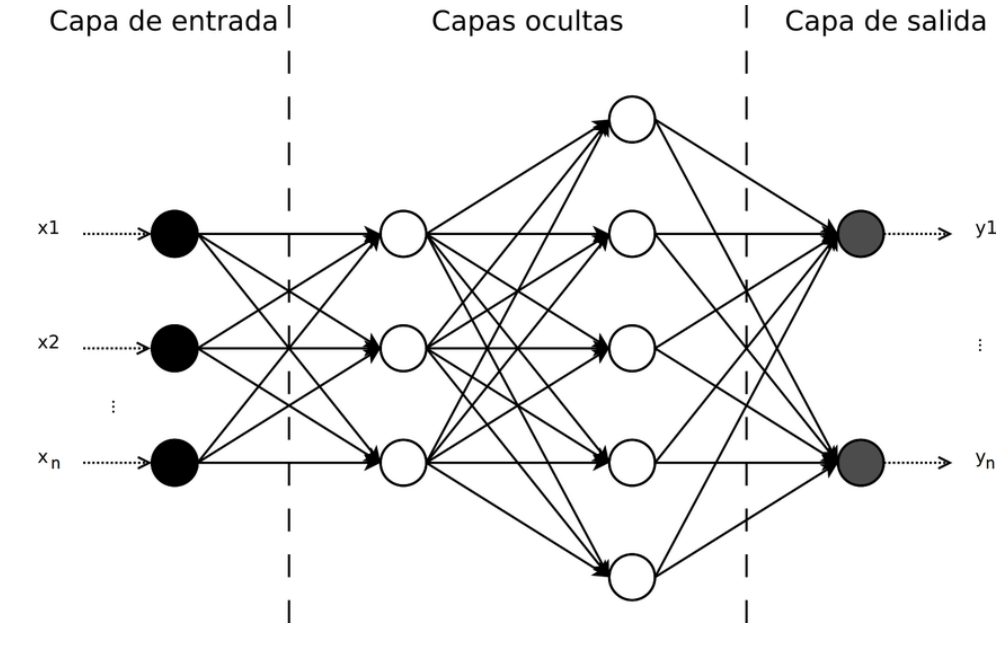
\includegraphics[width=0.5\textwidth]{Imagenes/fully_conected.png}
    \caption[Arquitectura de red neuronal \textit{fully connected}]{Esquema de una red
    neuronal \textit{fully connected}.}
    \label{fig:red_fc}
\end{figure}

El proceso de ajuste se lleva a cabo con TensorFlow \cite{TensorFlow}, una librería de Python de código abierto desarrollada por Google que proporciona herramientas de alto nivel para la definición, entrenamiento y exportación de modelos neuronales. Aun así, antes de definir la arquitectura de la red hay que recopilar una serie de datos que formaran el conjunto de entrenamiento.

\subsection{Dataset}

El \textit{dataset} es el conjunto de ejemplos etiquetados a partir del cual la red aprende a asociar cada combinación de lecturas sensoriales con la posición correcta de la mano. En este trabajo, las entradas de la red son los dos valores del \gls{adc}
correspondientes a los dedos índice y corazón, únicos sensores piezorresistivos destinados al reconocimiento de postura. Los dedos anular y meñique se reservan para funciones de control independientes descritas en la sección~\ref{sec:dron}, por lo que sus lecturas no forman parte del clasificador.

La salida de la red es un identificador de posición codificado como un entero entre
0 y 8, correspondiente a las 9 posiciones representadas en la
Figura~\ref{fig:posiciones_dataset}. Esta reducción respecto al trabajo previo, donde se usaban más dedos \cite{TFG}, podría suponer una limitación, pero en ciertos aspectos aporta ventajas sobre la red neuronal: con solo 2 entradas en lugar de 4, el espacio de estados que la red debe aprender es considerablemente más reducido, lo que permite alcanzar precisiones elevadas con arquitecturas más pequeñas, menor tiempo de inferencia en el microcontrolador y menor riesgo de sobreajuste durante el entrenamiento. Además, al disponer de un número de clases ligeramente menor (9 frente a 10), el problema de clasificación resulta intrínsecamente más sencillo, especialmente porque se eliminan algunas de las posiciones más similares entre sí que generan mayor confusión en la red.

\begin{figure}[htbp]
    \centering
    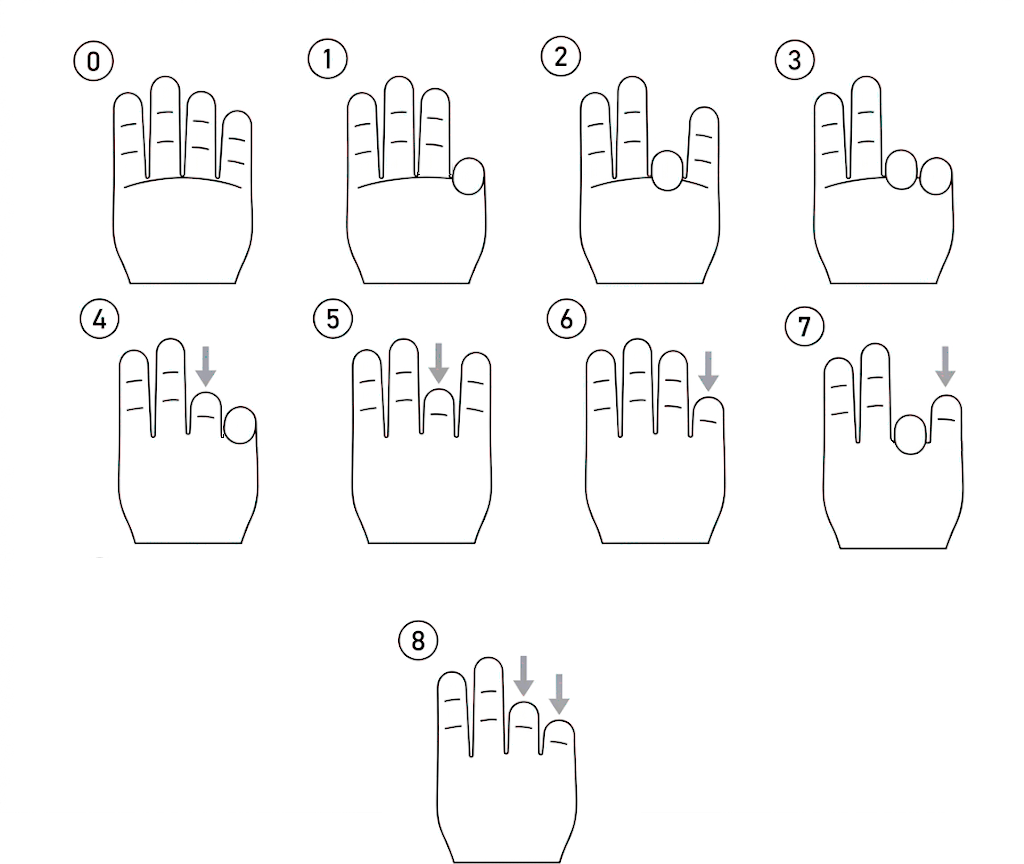
\includegraphics[width=0.5\textwidth]{Imagenes/DATASET.png}
    \caption[Posiciones definidas para el \textit{dataset}]{Representación de las 9
    posiciones definidas para el \textit{dataset}.}
    \label{fig:posiciones_dataset}
\end{figure}

Para la adquisición de los datos se desarrolló un programa que, cada vez que se pulsa \textit{enter}, solicita al usuario que adopte una de las posiciones indicadas y almacena las lecturas de los sensores en un fichero de texto. Con el fin de dotar a la red de la mayor robustez posible frente a variaciones en la colocación del guante o en las condiciones de uso, el \textit{dataset} se tomó a lo largo de varios días distintos, introduciendo así dispersión natural debida a ligeras diferencias en la posición del guante sobre la mano o en la postura del brazo.

El conjunto de datos resultante cuenta con aproximadamente XXX muestras por posición, distribuidas de forma uniforme entre las 9 clases para evitar sesgos durante el entrenamiento, como puede comprobarse en la Figura~\ref{fig:histograma_dataset}.
En cuanto al reparto, el 80\,\% de los datos se destinan al entrenamiento, el 10\,\% a la validación y el 10\,\% restante al test, seleccionados de forma aleatoria.

\begin{figure}[htbp]
    \centering
    % INSERTAR FIGURA: histograma de distribución del dataset por posición
    \caption[Distribución del \textit{dataset} por posición]{Histograma del número de
    muestras por posición en el \textit{dataset}.}
    \label{fig:histograma_dataset}
\end{figure}

\begin{figure}[htbp]
    \centering
    % INSERTAR FIGURA: gráficos de bigotes por dedo y posición
    \caption[Distribución de valores ADC por posición]{Gráficos de cajas y bigotes que
    muestran la distribución de los valores del \gls{adc} para cada dedo en cada
    posición del \textit{dataset}.}
    \label{fig:boxplot_dataset}
\end{figure}

Por conveniencia, los valores del \textit{dataset} se escalan acotando todas las lecturas entre 0 y 1 respecto a los extremos registrados durante una calibración previa.
Esta normalización garantiza que, aunque existan ligeras variaciones en el funcionamiento de los sensores entre sesiones o diferencias en la colocación del guante, el clasificador opere siempre sobre el mismo rango de entrada, preservando su precisión
en el uso cotidiano.

\subsubsection{\textit{One-hot encoding}}

Dado que se trata de un problema de clasificación multiclase, la salida de la red se
codifica mediante \textit{one-hot encoding} \cite{OneHot}. En lugar de representar
cada posición como un único entero, la red cuenta con 9 salidas, una por clase, y
proporciona como resultado un vector de probabilidades cuya componente de mayor valor
indica la posición estimada. Para ello, cada etiqueta numérica del \textit{dataset} se
sustituye por un vector de 9 elementos con un 1 en la posición correspondiente y 0 en
el resto. Así, por ejemplo, la posición 0 (mano abierta) queda codificada como
\texttt{100000000}, mientras que la posición 3 se representaría como \texttt{000100000}.

En la capa de salida, esta codificación se asocia habitualmente a la función de
activación \textit{softmax}, que mapea el vector de salida al simplex de probabilidades
garantizando que la suma de todas las componentes sea la unidad
(Figura~\ref{fig:activaciones}a). Sin embargo, esta función no está implementada en la
librería empleada para la exportación del modelo al microcontrolador. Por ello se
sustituye por la función ReLU (Figura~\ref{fig:activaciones}b), presente en el resto de
capas de la red, cuya sencillez la hace especialmente eficiente en hardware embebido.
Aunque con esta sustitución se pierde la interpretación probabilística estricta de la
salida, los resultados experimentales obtenidos resultan igualmente satisfactorios.

\begin{figure}[htbp]
    \centering
    % INSERTAR FIGURA: subfiguras con softmax y ReLU
    \caption[Funciones de activación]{Funciones de activación empleadas en la red:
    (a) \textit{Softmax}, usada habitualmente en la capa de salida de clasificadores
    multiclase. (b) ReLU, empleada en todas las capas de la red final.}
    \label{fig:activaciones}
\end{figure}

\subsection{Entrenamiento y selección de la arquitectura}

El objetivo del proceso de entrenamiento es encontrar la red de menor tamaño posible
que mantenga una precisión próxima al 100\,\%, ya que una red más compacta ocupa menos
memoria en el microcontrolador y reduce el tiempo de inferencia, aspecto crítico dado
el ciclo de 10\,ms impuesto por la tasa de muestreo de la \gls{imu}.

La red se fija en 4 capas: una capa de entrada de 2 neuronas, dos capas ocultas de
tamaño variable y una capa de salida de 9 neuronas. Se exploran distintas
configuraciones de las capas ocultas, evaluando cómo evoluciona la precisión en
validación al variar el número de neuronas en la primera capa oculta con la segunda
fijada en 15 neuronas (Figura~\ref{fig:precision_vs_neuronas}). A partir de los
resultados, se seleccionan únicamente las configuraciones que superan el 95\,\% de
precisión, lo que acota el rango de arquitecturas candidatas.

\begin{figure}[htbp]
    \centering
    % INSERTAR FIGURA: precisión vs. tamaño primera capa oculta
    \caption[Evolución de la precisión con el tamaño de la primera capa oculta]{Evolución
    de la precisión de la red en función del número de neuronas en la primera capa
    oculta, con la segunda capa fijada en 15 neuronas.}
    \label{fig:precision_vs_neuronas}
\end{figure}

Durante el entrenamiento se ajustan dos hiperparámetros adicionales: el número de
épocas y el \textit{dropout}. El número de épocas determina cuántas iteraciones
completas sobre el conjunto de entrenamiento realiza el optimizador; aunque aumentarlo
mejora la precisión, a partir de cierto punto la red queda atrapada en un óptimo local
y deja de mejorar. El \textit{dropout} mitiga este problema reiniciando aleatoriamente
una fracción de los pesos entre épocas, forzando a la red a explorar nuevas soluciones
y evitando el estancamiento. Con esta estrategia se alcanzan precisiones del 99\,\%,
a costa de tiempos de entrenamiento algo más prolongados.

\subsection{Compresión e integración con TensorFlow Lite}

Una vez seleccionada la arquitectura óptima, el modelo se exporta al microcontrolador
mediante TensorFlow Lite \cite{TFLite} y su adaptación para Arduino, la librería
Eloquent \cite{Eloquent}. El proceso de compresión consta de dos etapas: en primer
lugar, se congelan todos los pesos de la red convirtiéndolos de variables a constantes
y se elimina la arquitectura de entrenamiento, conservando únicamente la parte de
inferencia; en segundo lugar, los parámetros se cuantifican de punto flotante de 32
bits a punto fijo de 8 bits, reduciendo drásticamente el tamaño del modelo en memoria.

El resultado de la compresión es un fichero \texttt{.h} que se incorpora directamente
al programa del Arduino. Dado que la cuantificación puede degradar la precisión, se
evalúan todas las redes candidatas tras la compresión para identificar cuáles mantienen
su rendimiento. Se observa que las configuraciones con menor número de neuronas
presentan una mayor pérdida de precisión al comprimir, especialmente en la distinción
de posiciones similares entre sí. En cuanto a los tiempos de inferencia, la diferencia
entre la red más pequeña y la más grande es inferior a 0.1\,ms, por lo que se adopta
la red de mayor tamaño de entre las validadas, ya que ofrece la mayor robustez ante
posiciones próximas sin comprometer el ciclo temporal del sistema. La arquitectura
final seleccionada se muestra en la Figura~\ref{fig:arquitectura_red}.

\begin{figure}[htbp]
    \centering
    % INSERTAR FIGURA: tabla o esquema con capas, tamaños y número de parámetros
    \caption[Arquitectura final de la red neuronal]{Arquitectura de la red neuronal
    seleccionada tras el proceso de entrenamiento y compresión: tamaño de cada capa y
    número de parámetros entrenables.}
    \label{fig:arquitectura_red}
\end{figure}

Complementando al clasificador, se implementa un mecanismo de confirmación de posición:
el sistema solo registra un cambio de estado cuando la red predice la nueva posición de
forma consistente durante un intervalo de tiempo mínimo. Dado que el ciclo de medida
es de 10\,ms, significativamente inferior al tiempo de reacción motora del usuario,
sin este mecanismo las transiciones entre posiciones o los errores puntuales de la red
generarían detecciones espurias que degradarían la experiencia de control.


\section{Estudio de percepción de sensación táctil}

Con el hardware completamente ensamblado y el firmware de control operativo, el siguiente paso antes de integrar el sistema en la aplicación final es caracterizar y validar experimentalmente el módulo de estimulación electrotáctil. Este apartado recoge, en primer lugar, la caracterización eléctrica del circuito para establecer la relación entre la configuración del potenciómetro digital y la corriente realmente inyectada en los electrodos. A partir de dicha caracterización se obtiene una curva de linealización que permite programar directamente valores de corriente desde el microcontrolador. En segundo lugar, se describe un estudio perceptivo realizado sobre el propio autor con el objetivo de evaluar la capacidad del sistema para generar sensaciones táctiles localizadas en los puntos de la mano definidos en la sección~2.

\subsection{Caracterización de la curva de corriente}

El potenciómetro digital MAX5413 admite valores de configuración $P$ comprendidos entre 0 y 255, que el microcontrolador transmite mediante el protocolo SPI. Internamente, este dispositivo actúa como una resistencia variable en la red de polarización del amplificador operacional LMV342, de modo que el valor de $P$ determina la resistencia efectiva $R(P)$ del potenciómetro según la relación:

\begin{equation}
    R(P) = R_{\max} \cdot \frac{P}{255},
\end{equation}

donde $R_{\max}$ es la resistencia máxima del dispositivo, en este caso $10~\mathrm{k}\Omega$. Dado que el amplificador operacional junto con el transistor FET configura una fuente de corriente controlada por voltaje, la corriente de salida queda determinada por la tensión en el nodo de control, que a su vez es inversamente proporcional a $R(P)$. La corriente resultante sigue por tanto la relación:

\begin{equation}
    I(P) = \frac{Cte}{P},
    \label{eq:curva_corriente}
\end{equation}

donde $K$ es una constante que agrupa los parámetros del circuito. Esta dependencia hiperbólica implica que incrementos iguales de $P$ no producen incrementos iguales de corriente, siendo la respuesta muy sensible a valores bajos de $P$ y
progresivamente más plana a medida que $P$ aumenta.

Para verificar experimentalmente esta relación y cuantificar el valor de $K$, se conectó una resistencia de carga conocida $R_L=1000 ~\Omega$ entre los terminales de salida del circuito en lugar de los electrodos. Midiendo la tensión $V_L$ en bornes de la
resistencia con un multímetro, la corriente se obtiene directamente como $I = V_L / R_L$. El procedimiento se repitió para varios valores de $P$ entre 0 y 255, programando cada configuración desde el Arduino y registrando la medida correspondiente. Los resultados obtenidos se muestran en la
Figura~\ref{fig:curva_IP}.

\begin{figure}[htbp]
    \centering
        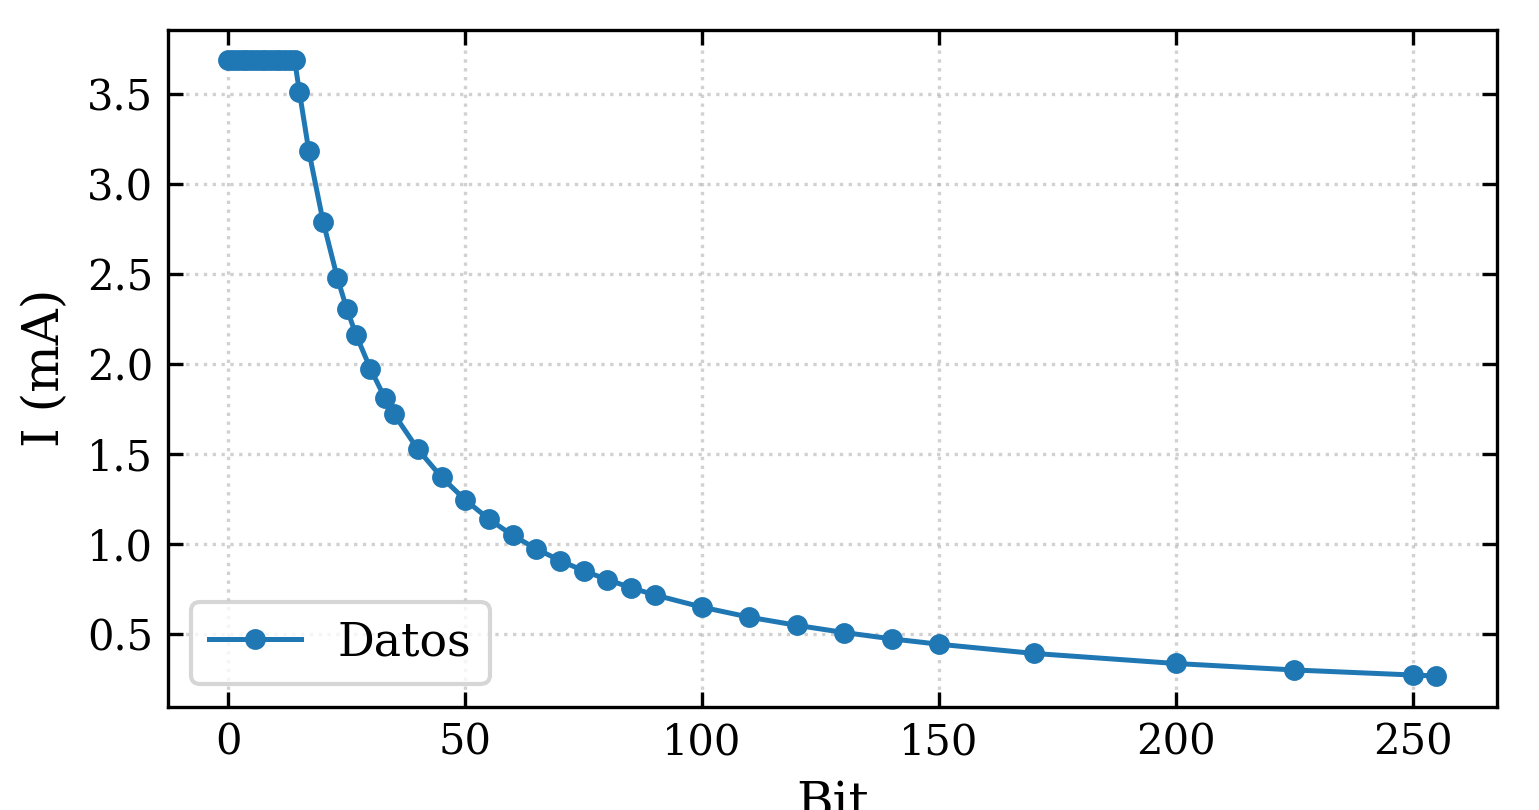
\includegraphics[width=0.8\textwidth]{Imagenes/curva_i_bit.png}
    \caption[Curva de corriente en función del valor del potenciómetro]{Corriente
    medida en la carga en función del valor de configuración $P$ del potenciómetro
    digital. La curva presenta la forma hiperbólica $I = Cte/P$ predicha, quitando la zona donde el diodo limitador de corriente empieza a tener efecto}
    \label{fig:curva_IP}
\end{figure}

\subsection{Linealización y regresión}

La relación hiperbólica de la ecuación~\eqref{eq:curva_corriente} resulta poco
conveniente para el control del sistema, por lo que para obtener mediante una formula a que corriente corresponde cada valor de P, se procede a linealizar la curva mediante el cambio de variable $y = 1/I$, de modo que la relación entre corriente y variable transformada es lineal:

\begin{equation}
    y =  K \cdot P
    \label{eq:linealizada}
\end{equation}

Sobre los datos experimentales transformados se realiza una regresión lineal por mínimos cuadrados, ajustando el modelo $y = a \cdot x + b$, donde el término independiente $b$ recoge posibles offset residuales del circuito. Los parámetros del ajuste obtenidos son:

\begin{equation}
    \hat{a} = 0.01441 \,\text{mA}, \qquad \hat{b} = 0.0824 \,\text{mA},
\end{equation}

con un coeficiente de determinación $R^2 = 0.9999$, lo que confirma la validez del modelo linealizado para describir el comportamiento del circuito en el rango de operación. Para el ajuste no se han tenido en cuenta los datos donde el diodo limitador de corriente tiene efecto. El ajuste se muestra superpuesto a los datos experimentales en la
Figura~\ref{fig:regresion}.

\begin{figure}[htbp]
    \centering
        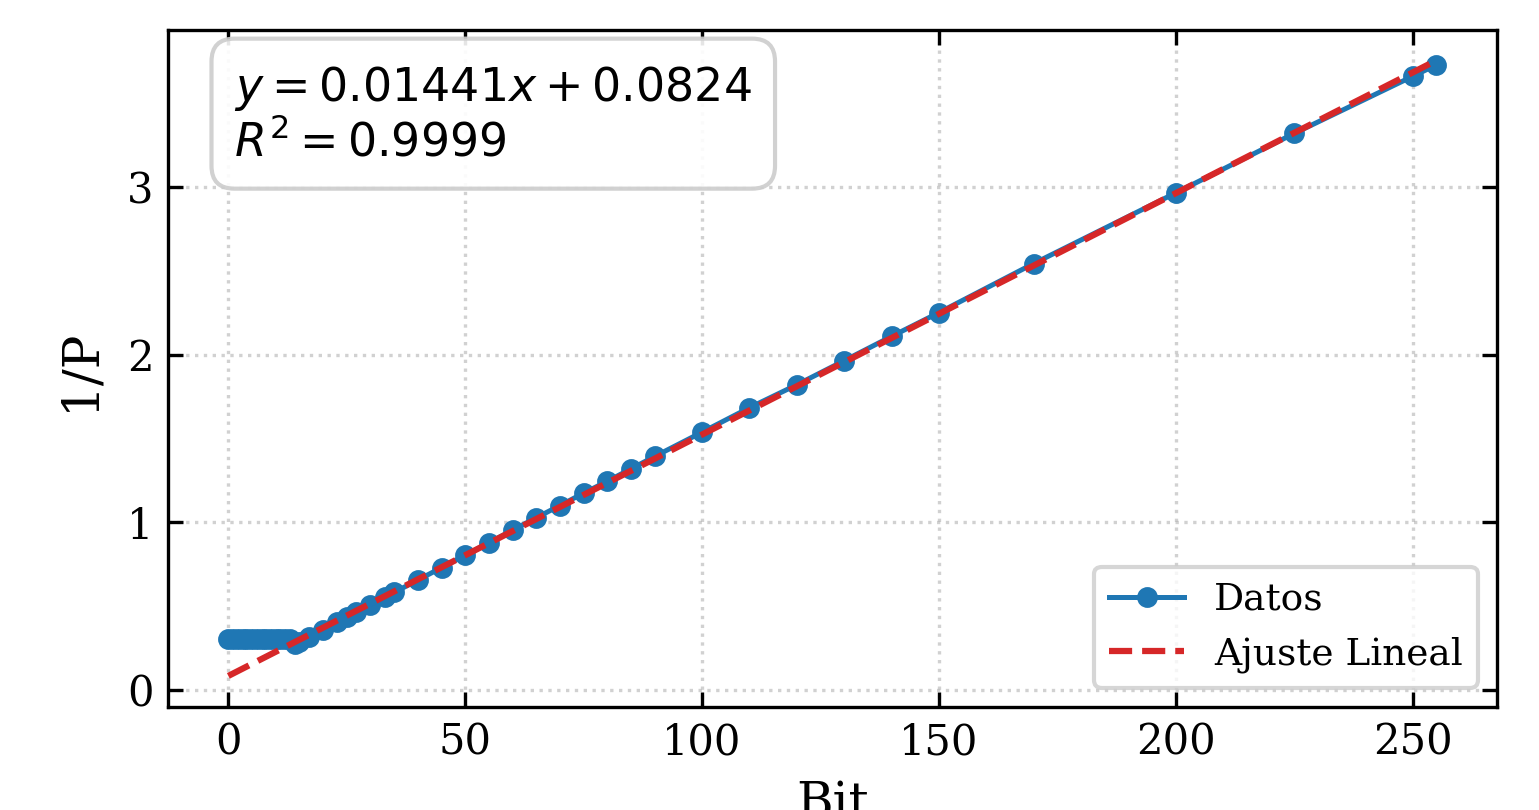
\includegraphics[width=0.8\textwidth]{Imagenes/curva_v_bit.png}
    \caption[Regresión lineal sobre la curva linealizada]{Corriente medida en función
    de $1/P$ junto con la recta de regresión obtenida por mínimos cuadrados. El
    elevado valor de $R^2$ confirma el comportamiento lineal tras el cambio de
    variable.}
    \label{fig:regresion}
\end{figure}

Por lo tanto, dado un valor de $P$ el circuito dará una corriente de salida que seguirá la ecuación \ref{eq:calibracion}:

\begin{equation}
    I(P)=\frac{1}{0,01441\cdot P+0,0824}~mA
    \label{eq:calibracion}
\end{equation}

que se implementa en el firmware del Arduino para traducir cualquier valor de bit programado que se envía por SPI al MAX5413 con el valor de corriente correspondiente . De este modo, el resto del sistema opera en unidades de miliamperios, desacoplando la lógica de control de los detalles del circuito analógico.

Como se observa en las dos figuras, el diodo limitador E-452 integrado en serie garantiza que, ante cualquier combinación de parámetros, la corriente que entra en el multiplexador no supere los 4.5\,mA, por lo que la ecuación~\eqref{eq:calibracion} solo es válida en el rango $P \in [15,\,255]$\,mA.
Los demás valores de $P$ tendrán una corriente muy parecida a la que corresponde a $P=15$

\subsection{Estudio perceptivo}

Con el circuito caracterizado, se procede a validar el sistema
háptico mediante un estudio de percepción que se realizará sobre el propio autor. El objetivo será comprobar mediante un estudio rápido cuáles de los diez canales de estimulación, y con que polarización, son capaces de generar una sensación referida a la zona palmar esperada, descartando aquellos en los que la localización o la sensación no sea la correcta. Para ver los resultados conseguidos por un sistema similar pero con un número mayor de pacientes, se puede consultar la referencia \cite{Tanaka2023}.

\subsubsection{Protocolo experimental}

Para el estudio se emplea la señal \textit{Burst}, un pulso cuadrado de 50\,ms en estado activo, que produce una sensación puntual comparable a la de pulsar un botón. Para cada canal, se parte de un valor de $P$ elevado, correspondiente a una corriente baja, y se va reduciendo progresivamente hasta que el autor detecta alguna sensación. En ese punto, se envian 5 pulsos consecutivos y se anota la zona de la mano en la que se ha percibido el estímulo. Si la zona indicada coincide con la zona palmar esperada para ese canal según el diseño de la sección~2, el canal se considera válido; en caso contrario, se descarta.

\subsubsection{Resultados}

La Tabla~\ref{tab:umbrales} recoge, para cada canal, la zona palmar objetivo, la polaridad de estimulación y el resultado del estudio. La Figura a la izquierda de la tabla muestra la correspondencia entre cada canal y su zona palmar asociada.
\newpage
\begin{table}[htbp]
    \centering
    \renewcommand{\arraystretch}{1.2}
    
    % --- COLUMNA IZQUIERDA: IMAGEN (a) ---
    \begin{subfigure}[b]{0.42\textwidth}
        \centering
        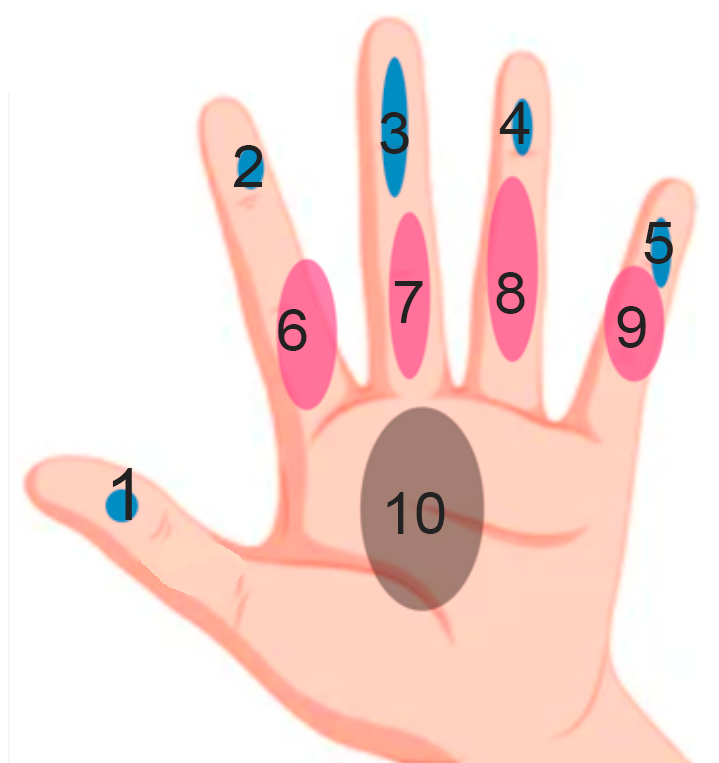
\includegraphics[width=\textwidth]{Imagenes/canal_estimulacion.png}
        \caption{Zonas palmares objetivo por canal.}
        \label{fig:zonas_canales}
    \end{subfigure}
    \hfill % Espacio entre la imagen y la tabla
    % --- COLUMNA DERECHA: TABLA (b) ---
    \begin{subtable}[b]{0.54\textwidth}
        \centering
        \small % Reducimos un poco el texto de la tabla si es necesario para que quepa al lado
        \begin{tabular}{clcc}
            \hline
            \textbf{Canal} & \textbf{Zona objetivo} & \textbf{Polaridad} & \textbf{Válido} \\
            \hline
            \multirow{2}{*}{ch1}  & \multirow{2}{*}{Pulgar}           & Anódica  & Dorsal \\
                                  &                                   & Catódica & \checkmark \\
            \arrayrulecolor{gray!40}\hline\arrayrulecolor{black}
            \multirow{2}{*}{ch2}  & \multirow{2}{*}{Índice distal}    & Anódica  & \checkmark \\
                                  &                                   & Catódica & Dorsal\\
            \arrayrulecolor{gray!40}\hline\arrayrulecolor{black}
            \multirow{2}{*}{ch3}  & \multirow{2}{*}{Corazón distal}   & Anódica  & \checkmark \\
                                  &                                   & Catódica & Dorsal \\
            \arrayrulecolor{gray!40}\hline\arrayrulecolor{black}
            \multirow{2}{*}{ch4}  & \multirow{2}{*}{Anular distal}    & Anódica  & \checkmark \\
                                  &                                   & Catódica & \checkmark\\
            \arrayrulecolor{gray!40}\hline\arrayrulecolor{black}
            \multirow{2}{*}{ch5}  & \multirow{2}{*}{Meñique distal}   & Anódica  & \checkmark \\
                                  &                                   & Catódica & Dorsal\\
            \arrayrulecolor{gray!40}\hline\arrayrulecolor{black}
            \multirow{2}{*}{ch6}  & \multirow{2}{*}{Índice proximal}  & Anódica  & \checkmark\\
                                  &                                   & Catódica & Dorsal\\
            \arrayrulecolor{gray!40}\hline\arrayrulecolor{black}
            \multirow{2}{*}{ch7}  & \multirow{2}{*}{Corazón proximal} & Anódica  & \checkmark \\
                                  &                                   & Catódica & 50/50 \\
            \arrayrulecolor{gray!40}\hline\arrayrulecolor{black}
            \multirow{2}{*}{ch8}  & \multirow{2}{*}{Anular proximal}  & Anódica  & \checkmark \\
                                  &                                   & Catódica & 50/50\\
            \arrayrulecolor{gray!40}\hline\arrayrulecolor{black}
            \multirow{2}{*}{ch9}  & \multirow{2}{*}{Meñique proximal} & Anódica  & \checkmark \\
                                  &                                   & Catódica & 50/50 \\
            \arrayrulecolor{gray!40}\hline\arrayrulecolor{black}
            \multirow{2}{*}{ch10} & \multirow{2}{*}{Palma}            & Anódica  & $\times$ \\
                                  &                                   & Catódica & \checkmark \\
            \hline
        \end{tabular}
        \caption{Validación perceptiva.}
        \label{tab:umbrales_datos}
    \end{subtable}

    \vspace{10pt} % Espacio entre los elementos y el caption principal
    % --- CAPTION PRINCIPAL DETALLADO ---
    \caption[Estudio de localización y validación por canal]{Estudio de localización del estímulo: 
    \textbf{a)} Zonas palmares correspondientes a cada canal de estimulación. 
    \textbf{b)} Resultado del estudio de localización para cada canal y polaridad de estimulación. La columna \textit{Válido} indica si la sensación referida coincidió con la zona esperada (\checkmark), si se percibió en la zona Dorsal, si se percibió en ambas partes (50/50), o si no se percibió ninguna sensación ($\times$).}
    \label{tab:umbrales}
\end{table}

Los canales que superaron la validación concuerdan con el mecanismo de sensaciones referidas descrito en la sección~2: la estimulación aplicada en el dorso de la mano se percibe en la zona palmar correspondiente, y no en la zona dorsal donde se sitúan los electrodos. Para estos canales, se anota que la corriente promedia donde se empezó a notar sensación táctil, fue de $3.38~mA$, cifra algo elevada puesto que se acerca al umbral de máxima corriente impuesto.
Los canales descartados corresponden en su mayoría a zonas anatómicamente próximas entre sí, donde la separación inter-electrodo no es suficiente para aislar completamente la corriente hacia el nervio digital objetivo. Este resultado está en línea con las limitaciones del sistema de doble tierra discutidas en la sección~2, y determina el subconjunto de canales que se podrán emplear en la aplicación de control de la sección~\ref{sec:dron}.

% ==============================================================
% SECCIÓN: Control de dron como aplicación del sistema háptico
% ==============================================================

\section{Aplicación del sistema: control de un dron con feedback háptico}
\label{sec:dron}

Como aplicación del sistema desarrollado, para poner a prueba todo el trabajo en su conjunto, se decidió implementarlo como método de control de vuelo de un dron comercial de bajo coste, concretamente el modelo Karuisrc K417, empleando el guante como dispositivo de mando. La elección de esta plataforma responde a que el vuelo de un dron requiere gestionar de forma simultánea cuatro grados de libertad: aceleración, guiñada (\textit{yaw}), cabeceo (\textit{pitch}), alabeo (\textit{roll}). Esto es útil para obligar a activar en paralelo todos los subsistemas del guante: la estimación de orientación mediante el filtro de Mahony, la lectura de los sensores de flexión, el reconocimiento gestual mediante la red neuronal embebida y la retroalimentación háptica electrotáctil. El resultado es un bucle de control en el que el piloto actúa sobre el dron inclinando y girando la mano, mientras usa la posición de los dedos como canal adicional de control, a la vez que el sistema le devuelve información táctil localizada sobre la maniobra que está ejecutando, sin recurrir a ningún tipo de retroalimentación visual del estado del vuelo.

% ------------------------------------------------------------------
\subsection{Protocolo WiFi de control del dron}
\label{sec:dron_protocolo}
% ------------------------------------------------------------------

Para poder mandar ordenes al dron, se usa su punto de acceso Wi-Fi propio, pero el problema es que no dispone de documentación pública sobre su protocolo de comunicación. Para poder controlarlo desde el microcontrolador fue necesario caracterizar dicho protocolo mediante la técnica de captura de tráfico en red local. El procedimiento consistió en conectar un ordenador a la misma red inalámbrica que la aplicación para Android del dron y, mediante scripts desarrollados en Node.js y Python (disponibles en el Anexo \ref{Anexo:A}), interceptar y registrar todos los datagramas UDP que la app enviaba hacia la dirección IP del dron (\texttt{192.168.169.1}) a través del puerto 8800. Actuando sobre los controles de la aplicación de forma sistemática y observando simultáneamente cómo cambiaba el contenido de los paquetes capturados, fue posible asociar cada campo de la trama binaria a la función de vuelo correspondiente.

El análisis reveló que cada mensaje de control tiene una longitud fija de 124 bytes y está estructurado en cuatro bloques lógicos separados por campos de verificación y contadores de secuencia. La Tabla~\ref{tab:pkt_estructura} resume la organización del datagrama identificada en este proceso.

\begin{table}[htbp]
\centering
\caption{Estructura del datagrama UDP de 124 bytes del protocolo K417.}
\label{tab:pkt_estructura}
\begin{tabular}{clcc}
\hline
\textbf{Bloque} & \textbf{Contenido} & \textbf{Bytes} & \textbf{Naturaleza} \\
\hline
Cabecera        & Identificador de sincronización            & 12 & Fijo \\
C1              & Ejes de control + comando + \textit{headless} & 32 & Variable \\
\textit{Checksum} & Prefijo fijo + contadores de secuencia   & 14 & Variable \\
C2              & Repetición de ejes + campos de estado      & 32 & Variable \\
C3              & Información de estado adicional            & 34 & Variable \\
\hline
\textbf{Total}  &                                            & \textbf{124} & \\
\hline
\end{tabular}
\end{table}

\begin{table}[htbp]
\centering
\caption{Estructura del datagrama UDP de 124 bytes del protocolo K417.}
\label{tab:pkt_estructura2}
\resizebox{\textwidth}{!}{%
\begin{tabular}{clccp{6cm}}
\hline
\textbf{Bloque} & \textbf{Contenido} & \textbf{Bytes} & \textbf{Naturaleza} & \textbf{Detalle} \\
\hline
Cabecera & Identificador de sincronización & 12 & Fijo & \texttt{0xEF 0x02 0x7C \ldots} constante en todos los paquetes \\
\hline
\multirow{6}{*}{C1} & Alabeo, cabeceo, acelerador, guiñada & 4 & Variable & Enteros sin signo en [40,\,220]; neutro = 128 \\
                    & Comando especial & 1 & Variable & 0x00 normal, 0x01 despegue, 0x02 aterrizaje/parada, 0x04 calibración, 0x05 cámara \\
                    & Modo sin cabeza  & 1 & Variable & 0x02 off, 0x03 on; OR 0x08 activa acrobacia en ambos bytes \\
                    & Relleno          & 10 & Fijo    & Ceros \\
                    & \textit{Checksum} & 1 & Variable & XOR de los 6 bytes de control anteriores \\
                    & Sufijo           & 6 & Fijo     & \texttt{0x00 0x00 0x14 0x00 0x66 0x14} \\
\hline
Checksum & Prefijo fijo + contadores de secuencia & 14 & Variable & Tres contadores de 16 bits (\texttt{ctr1, ctr2, ctr3}) que se incrementan en cada envío \\
\hline
C2 & Contador \texttt{ctr2} + sufijo fijo & 32 & Variable & 
    Primeros 2 bytes: contador de secuencia; resto fijo (\texttt{C2\_SUFFIX}) \\
C3 & Contador \texttt{ctr3} + sufijo fijo & 34 & Variable & 
    Primeros 2 bytes: contador de secuencia; resto fijo (\texttt{C3\_SUFFIX}) \\
\hline
\textbf{Total} & & \textbf{124} & & \\
\hline
\end{tabular}%
}
\end{table}

Dentro del bloque C1 se sitúan los cuatro bytes de ejes de vuelo, cada uno codificado como un entero sin signo en el rango $[40,\,220]$, donde el valor 128 representa el punto neutro. El mismo bloque alberga un byte de comando especial, que puede tomar valores predefinidos para ordenar el despegue automático, el aterrizaje, la calibración de la \gls{imu} interna del dron, el movimiento de la cámara o el inicio de una acrobacia, y un byte de modo sin cabeza (\textit{headless}), que controla si el dron interpreta los ejes de traslación respecto a su propia orientación instantánea o respecto a la que tenía en el momento del despegue. Los bloques C2 y C3 repiten parte de la información de vuelo con campos de estado adicionales y cierran el datagrama con un sufijo de bytes de valor fijo que actúa como delimitador. La Tabla~\ref{tab:pkt_comandos} recoge los valores del byte de comando especial identificados durante la captura y su significado.

\begin{table}[htbp]
\centering
\caption{Valores del byte de comando especial en el bloque C1 del protocolo K417.}
\label{tab:pkt_comandos}
\begin{tabular}{cll}
\hline
\textbf{Valor (hex)} & \textbf{Constante en firmware} & \textbf{Acción} \\
\hline
\texttt{0x00} & \texttt{CMD\_NONE}        & Ninguna (control normal)    \\
\texttt{0x01} & \texttt{CMD\_TAKEOFF}     & Despegue automático         \\
\texttt{0x02} & \texttt{CMD\_LAND}        & Aterrizaje suave   \\
\texttt{0x04} & \texttt{CMD\_CALIBRATE}   & Calibración de la IMU del dron \\
\texttt{0x05} & \texttt{CMD\_STOP}     & Parar motores              \\
\texttt{0x08} & \texttt{SOMERSAULT\_FLAG} & Activar modo acrobacia) \\
\hline
\end{tabular}
\end{table}

% ------------------------------------------------------------------
\subsection{Bucle de control}
\label{sec:dron_bucle}
% ------------------------------------------------------------------

La totalidad del procesamiento se ejecuta en el microcontrolador Arduino Nano RP2040 Connect sin intervención de ningún sistema externo. El bucle principal opera a dos cadencias independientes: los paquetes de control se envían al dron a 40~Hz y la telemetría de diagnóstico se emite por el puerto serie a 25~Hz, evitando así que la carga de comunicación serie interfiera con el lazo de vuelo. La Figura~\ref{fig:dron_bucle} ilustra el flujo completo de procesamiento en cada iteración.

% ---- FIGURA: diagrama de flujo del bucle de control ----
\begin{figure}[htbp]
  \centering
  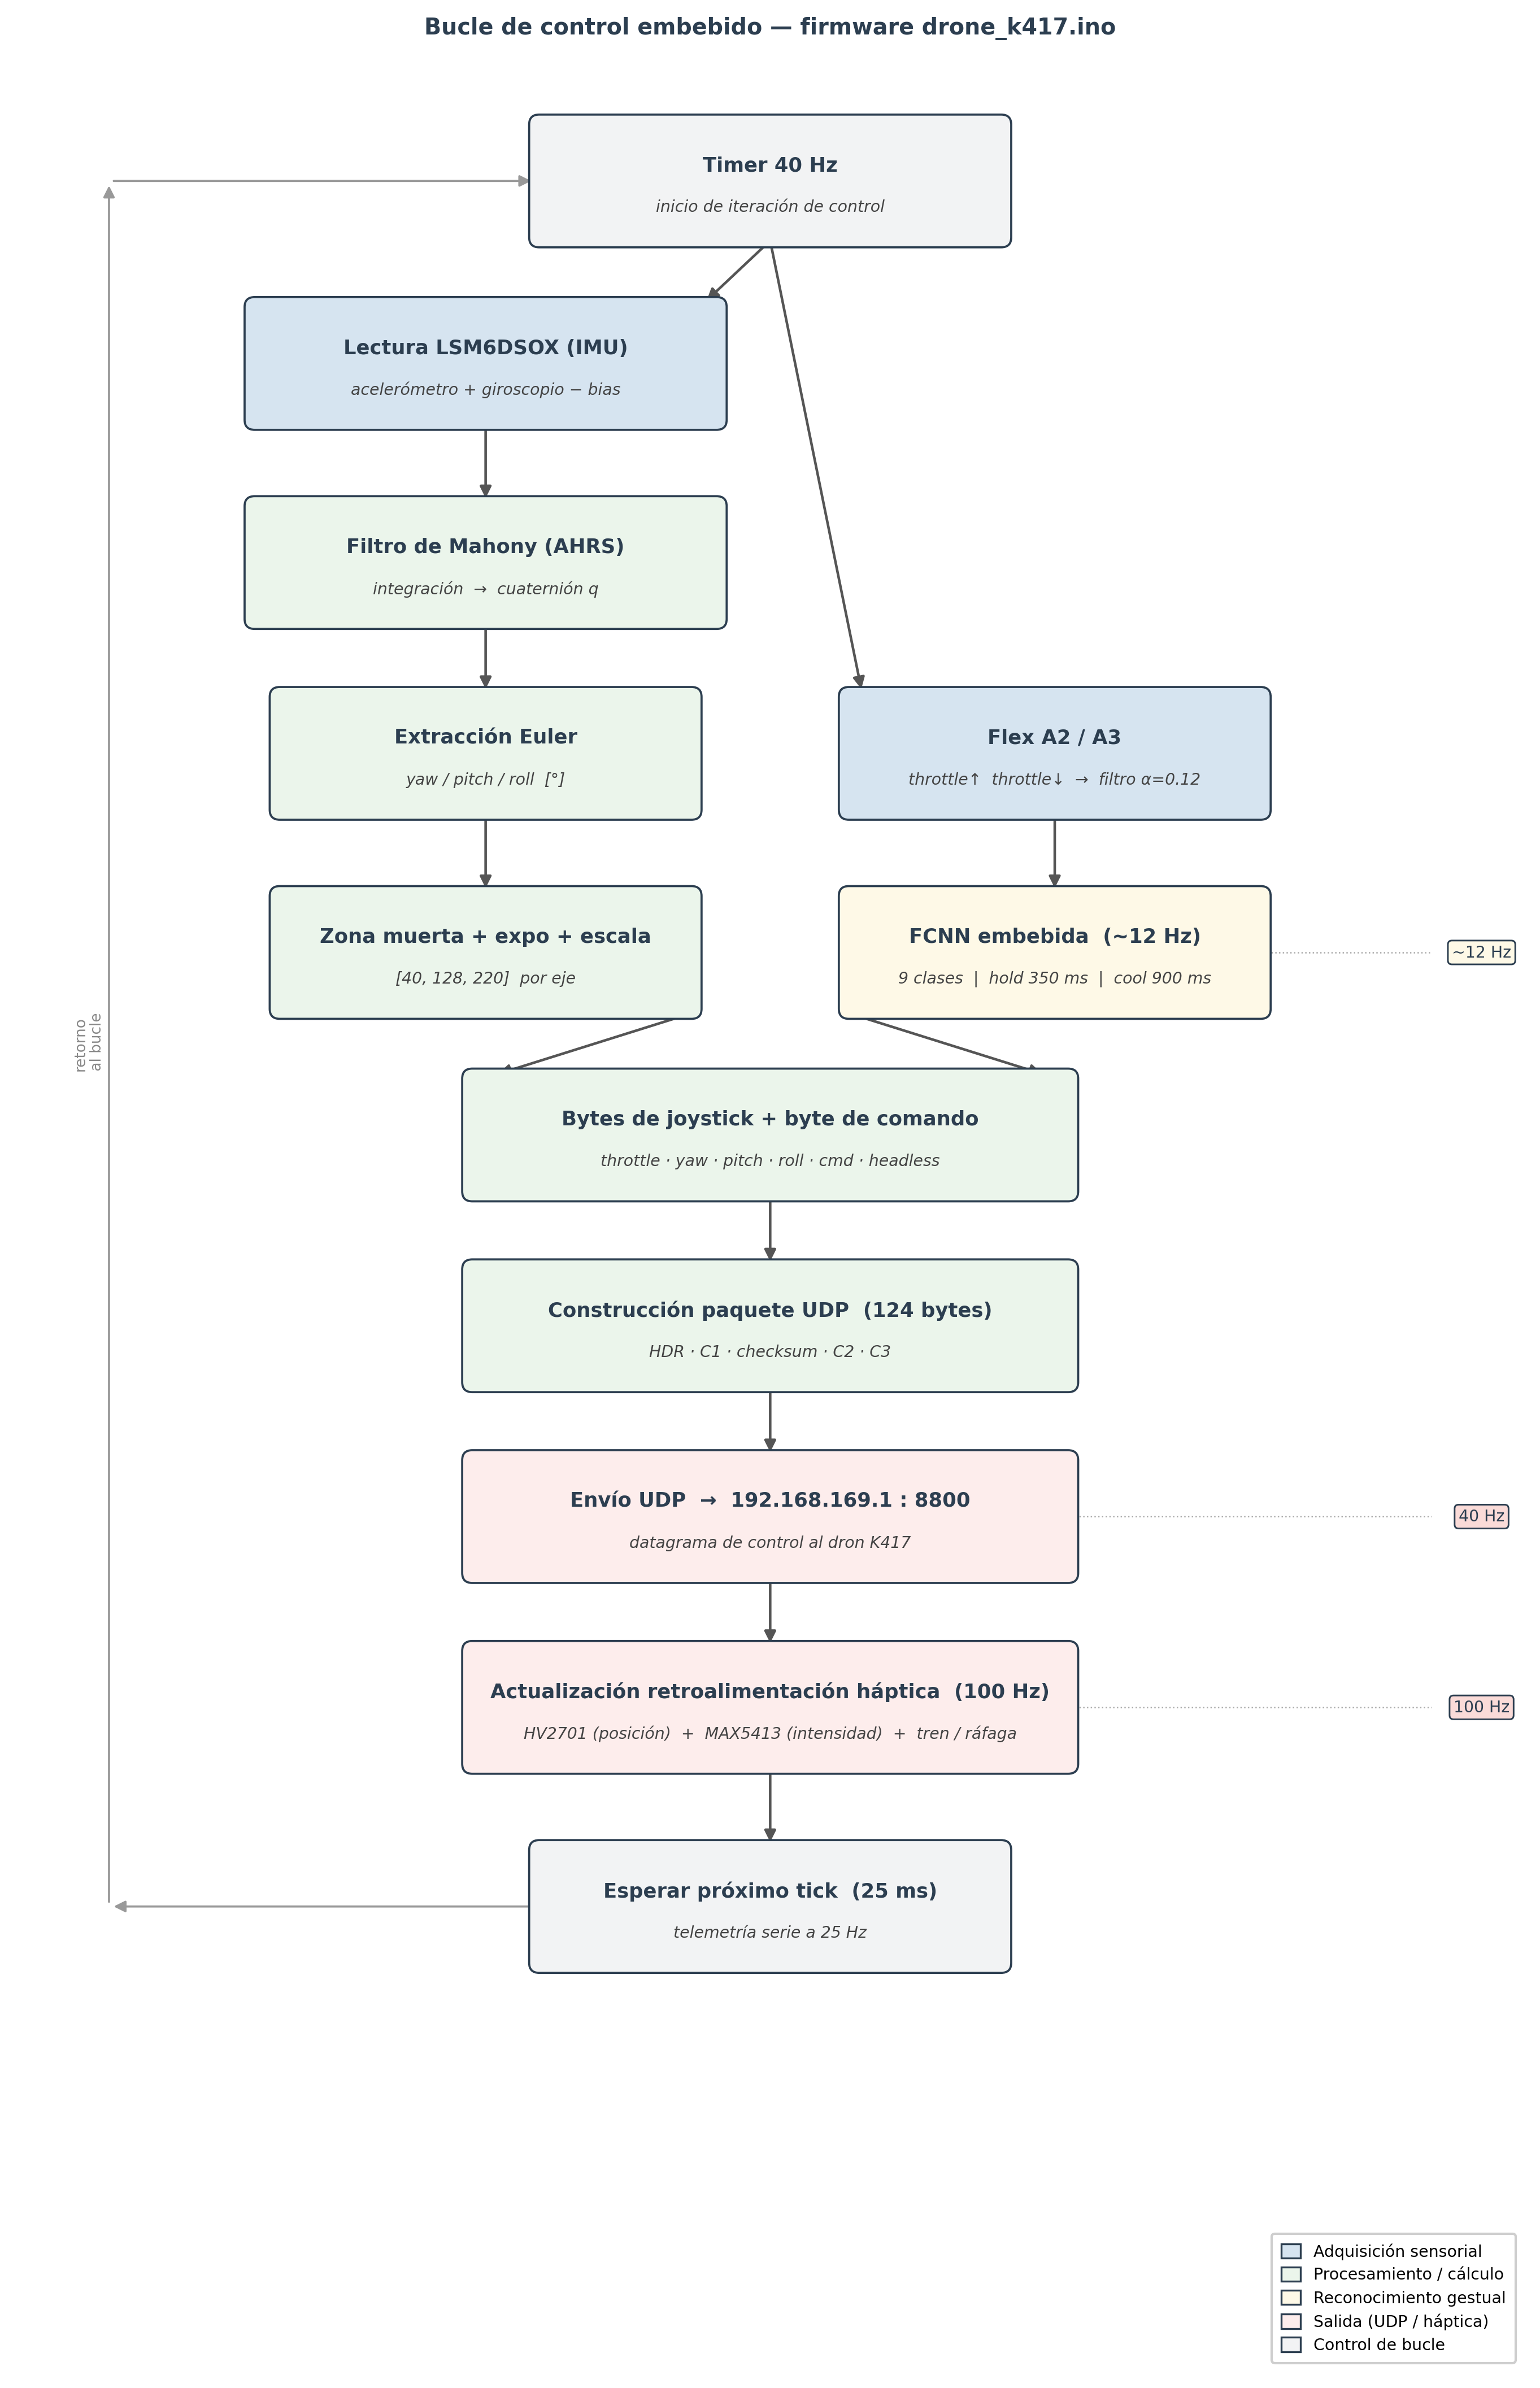
\includegraphics[width=0.82\textwidth]{Imagenes/dron_bucle_control}
  \caption{Diagrama de flujo del bucle de control embebido ejecutado a 40~Hz.}
  \label{fig:dron_bucle}
\end{figure}

\paragraph{Estimación de orientación.}
Al inicio de cada iteración se leen las medidas de acelerómetro y giroscopio del sensor LSM6DSOX y se integran en el filtro de Mahony para actualizar el cuaternión de orientación. Durante la fase de calibración inicial, que comprende 200 muestras tomadas con el guante en reposo, se estiman y corrigen los sesgos de \textit{offset} del giroscopio. El filtro opera con ganancia proporcional $K_p = 3{,}5$ y ganancia integral $K_i = 0{,}03$, valores que garantizan una convergencia rápida de la estimación frente a las perturbaciones de aceleración lineal que se producen durante el movimiento de la mano.

\paragraph{Mapeo de orientación a ejes de vuelo.}
A partir del cuaternión se extraen los ángulos de Euler de guiñada, cabeceo y alabeo. Antes de convertirlos en los bytes del joystick virtual se aplica sobre cada eje una cadena de acondicionamiento en tres etapas: una zona muerta de $8°$ que cancela las desviaciones de orientación menores para suprimir el temblor fisiológico de la mano; una función de exposición no lineal que suaviza la respuesta en torno al punto neutro y la amplifica en los extremos del recorrido; y un escalado lineal que convierte el ángulo resultante, acotado a un máximo de $45°$, al rango entero $[40,\,220]$ con 128 como valor neutro.

\paragraph{Control del acelerador mediante sensores de flexión.}
El canal de acelerador no se deriva de la orientación de la mano sino de dos sensores de flexión dedicados, conectados a las entradas analógicas A2 (gas positivo) y A3 (gas negativo). La diferencia entre sus lecturas normalizadas, calculada respecto a la media y desviación típica registradas durante la calibración, se filtra mediante un promedio exponencial de primer orden con coeficiente $\alpha = 0{,}12$ para eliminar transitorios bruscos y se mapea al mismo rango $[40,\,220]$.

\paragraph{Reconocimiento gestual y comandos discretos.}
La red neuronal \textit{fully-connected} embebida procesa a aproximadamente 12~Hz las lecturas normalizadas de los cuatro sensores de flexión y produce una estimación de la clase gestual activa entre nueve posibles. Para reducir la tasa de falsos positivos, el firmware exige que la clase predicha se mantenga estable durante al menos 350~ms y que el margen de confianza supere un umbral mínimo antes de activar el comando de vuelo asociado. Una vez disparado un comando, se impone un período de bloqueo de 900~ms durante el cual no puede activarse ninguna acción nueva. La Tabla~\ref{tab:nn_gestos} relaciona las clases gestuales con los comandos de vuelo y el patrón de retroalimentación háptica emitido como confirmación.

\begin{table}[htbp]
\centering
\caption{Correspondencia entre clase gestual, comando de vuelo y retroalimentación háptica de confirmación.}
\label{tab:nn_gestos}
\begin{tabular}{clll}
\hline
\textbf{Clase} & \textbf{Comando de vuelo} & \textbf{Zona háptica} & \textbf{Modo} \\
\hline
0 & Reposo (sin acción)                        & ---                 & ---            \\
1 & Despegue automático                        & Palma (M20)         & Ráfaga $\times 1$ \\
2 & Aterrizaje suave                           & Palma (M20)         & Ráfaga $\times 1$ \\
3 & Parada de emergencia                       & Palma (M20)         & Ráfaga $\times 3$ \\
4 & Calibración IMU dron                       & Índice (M8)         & Ráfaga $\times 1$ \\
5 & Activar/desactivar modo \textit{headless}  & Pulgar (M4)         & Ráfaga $\times 1$ \\
6 & Elevar cámara                              & Índice (M8)         & Ráfaga $\times 1$ \\
7 & Acrobacia (\textit{flip})                  & Medio-anular (M12)  & Ráfaga $\times 3$ \\
8 & Modo acrobacia latente                     & ---                 & ---            \\
\hline
\end{tabular}
\end{table}

% ------------------------------------------------------------------
\subsection{Secuencia de acrobacia}
\label{sec:dron_flip}
% ------------------------------------------------------------------

La maniobra de acrobacia merece una descripción específica por su mayor complejidad temporal. Cuando el gesto correspondiente supera los umbrales de estabilidad y confianza, el firmware congela los valores actuales de los cuatro ejes de vuelo y entra en una máquina de estados de dos fases. Durante la primera fase, denominada de impulso, se envían 20 paquetes consecutivos con el indicador de acrobacia activado en el byte de comando y el acelerador forzado a 212 sobre el máximo de 220, con el fin de dotar al dron del empuje necesario para completar el giro. Superado ese bloque de paquetes, se entra en la fase de recuperación, en la que se envían 10 paquetes adicionales con el acelerador reducido a 204 para estabilizar el vuelo antes de devolver el control al lazo normal. Durante las dos fases, los ejes de traslación permanecen congelados en los valores previos para impedir que movimientos involuntarios de la mano generen comandos espurios durante la maniobra.

% ------------------------------------------------------------------
\subsection{Retroalimentación háptica durante el vuelo}
\label{sec:haptic_drone}
% ------------------------------------------------------------------

La retroalimentación háptica cierra el lazo sensoriomotor informando al piloto, a través de la estimulación electrotáctil, sobre el estado de cada uno de los ejes de vuelo que está generando con la mano. El principio de diseño adoptado establece una correspondencia unívoca entre eje de control y zona anatómica, de modo que el piloto puede distinguir táctilmente qué canal está activo sin necesidad de apartar la vista del dron. La Tabla~\ref{tab:haptic_mapeo} resume esta correspondencia junto con los parámetros de estimulación empleados en cada canal, y la Figura~\ref{fig:dron_mapa_haptico} ilustra la distribución de las zonas sobre el dorso de la mano.

\begin{table}[htbp]
\centering
\caption{Correspondencia entre eje de vuelo, zona anatómica y parámetros del canal háptico.}
\label{tab:haptic_mapeo}
\begin{tabular}{lllcc}
\hline
\textbf{Eje de vuelo} & \textbf{Zona anatómica} & \textbf{Posición HV2701} & \textbf{Pot. mín.} & \textbf{Pot. máx.} \\
\hline
Guiñada (\textit{yaw})         & Región del pulgar      & M4  (canal 2)  & 16 & 25 \\
Cabeceo (\textit{pitch})       & Región del índice      & M8  (canal 3)  & 23 & 28 \\
Alabeo (\textit{roll})         & Región medio-anular    & M12 (canal 4)  & 28 & 35 \\
Acelerador (\textit{throttle}) & Región de la palma     & M20 (canal 10) & 14 & 20 \\
\hline
\end{tabular}
\end{table}

% ---- FIGURA: mapa anatómico de estimulación ----
% Sustituir el bloque \fbox por \includegraphics cuando la figura esté disponible.
\begin{figure}[htbp]
  \centering
  % \includegraphics[width=0.52\textwidth]{Imagenes/dron_mapa_haptico}
  \fbox{\parbox{0.52\textwidth}{\centering\vspace{2.5cm}
    [FIGURA: Dorso de la mano con las cuatro zonas de estimulación\\
    electrotáctil señaladas:\\
    pulgar $\leftrightarrow$ yaw, índice $\leftrightarrow$ pitch,\\
    medio-anular $\leftrightarrow$ roll, palma $\leftrightarrow$ throttle.]
  \vspace{2.5cm}}}
  \caption{Distribución de las cuatro zonas de retroalimentación háptica sobre el dorso de la mano para el control del dron.}
  \label{fig:dron_mapa_haptico}
\end{figure}

El sistema de retroalimentación opera a una cadencia de actualización de 100~Hz. En cada ciclo el firmware normaliza el valor de cada eje al rango $[0,\,1]$ y evalúa si supera el umbral neutro. Si al menos uno de los cuatro ejes está activo, se selecciona mediante un esquema de turno rotatorio el canal correspondiente: se escribe la palabra de 16 bits de la posición elegida en el HV2701 para conectar los electrodos de esa zona, se ajusta el potenciómetro digital MAX5413 al valor de intensidad asignado a ese canal y se lanza un tren de pulsos de 100~Hz con una anchura de pulso de 400~µs y una duración de 2~s. El esquema rotatorio garantiza que ningún canal monopolice el hardware de estimulación cuando varios ejes están activos de forma simultánea. Si todos los ejes vuelven a la posición neutra, la estimulación se detiene inmediatamente.

Para los comandos discretos generados por reconocimiento gestual se emplea una modalidad diferente: una ráfaga corta de pulsos en la zona anatómica asociada al gesto activado, cuyo número varía según la relevancia del comando. Una ráfaga de un pulso confirma comandos habituales como el despegue o el aterrizaje, mientras que una ráfaga de tres pulsos se reserva para maniobras de mayor impacto, como la parada de emergencia o la acrobacia, lo que permite al piloto distinguirlas táctilmente sin ambigüedad. Durante el tiempo que dura la ráfaga, un temporizador de bloqueo impide que el canal de retroalimentación continua se active, evitando solapamientos entre los dos modos de estimulación. Por último, durante la ejecución de la secuencia de acrobacia, toda la retroalimentación háptica se suspende de forma completa, dado que los ejes de control se encuentran artificialmente congelados y cualquier estímulo generado en ese instante carecería de correlación con el estado real del vuelo.

\begin{table}[htbp]
\centering
\caption{Desglose de tiempos de ejecución de un ciclo completo de programa.}
\label{tab:tiempos_bucle_horizontal}
\resizebox{\textwidth}{!}{% 
\begin{tabular}{|l|c|c|c|c|c|c|c|c|}
\hline
\rowcolor{light-gray} & \textbf{IMU (Lectura y Filtro)} & \textbf{ADC} & \textbf{Red Neuronal} & \textbf{Lógica CPU} & \textbf{Envío WiFi} & \textbf{Hápticos} & \textbf{Otros} & \textbf{TOTAL} \\ \hline
\textbf{Tiempo (ms)} & 3.494 & 0.083 & 1.415 & 0.212 & 2.115 & 0.403 & 0.039 & \textbf{6.880} \\ \hline
\end{tabular}% <--- ¡Llave corregida aquí!
}
\end{table}

\section{Conclusiones y trabajo futuro}

Se acabo el master


%------------------ BIBLIOGRAFÍA ------------------
\newpage
\bibliographystyle{unsrt}
\bibliography{Bibliografia_TFM}

%------------------ ANEXOS ------------------
\newpage
\pagenumbering{roman}
\section*{Anexos}



\begin{appendices}

\section{Repositorio de Git-Hub}
\label{Anexo:A}
\lipsum[2]

\section{GUI de control del dron}
\lipsum[3]

\end{appendices}

\end{document}